% Chapter 3

\chapter{Diseño e implementación} % Main chapter title

\label{Chapter3} % For referencing the chapter elsewhere, use \ref{Chapter3} 
\label{implementacion}

%----------------------------------------------------------------------------------------

\section{Solución propuesta}

En esta sección se dará una descripción general del sistema y las tecnologías que se utilizarán para este trabajo.

\subsection{Descripción general del sistema}

El hardware necesario para construir un dispositivo de eye-tracking se puede resumir en tres partes principales:

\begin{itemize}

\item Una \keyword{cámara} para captar movimientos oculares.

\item Un \keyword{procesador} que cumpla múltiples funciones. Entre ellas, analizar la imagen, determinar la dirección hacia la que el usuario está mirando y correr una aplicación de software interactiva con estos movimientos.

\item Una \keyword{pantalla o monitor} que se comunique con el procesador para mostrar la interfaz de la aplicación.

Para nuestro trabajo se necesita de una cuarta parte adicional, que engloba a todos los dispositivos periféricos necesarios para que los examinadores, compañeros o familiares puedan personalizar las preguntas que se le realizan al estudiante (se aclaró previamente que, junto al monitor, lo proveerán los dispositivos externos). A grandes rasgos, el sistema se resume en el diagrama de la figura \ref{fig:bloques1}.

\begin{figure}[htbp]
    \centering
    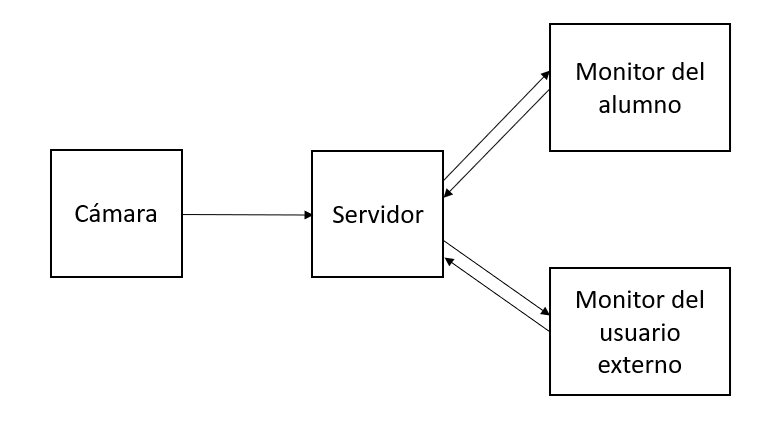
\includegraphics[width=0.5\textwidth]{figuras/bloques1.png}
    \caption{Diagrama de bloques general del sistema}
    \label{fig:bloques1}
\end{figure}

En cuanto a los requisitos de software, se necesita que el dispositivo pueda almacenar información de usuarios, preguntas y respuestas en una base de datos propia, para que cualquier usuario registrado pueda informarse respecto al rendimiento académico del estudiante que lo utilizará.
Una vez establecidos los requisitos mínimos, se describe a continuación cómo funcionará nuestro sistema.

El núcleo central de nuestro trabajo se basa en el uso de un microcontrolador de bajo costo, que será el encargado de realizar todo el procesamiento de imagen y aplicaciones anteriormente descrito. Naturalmente, sus capacidades de memoria y procesamiento son limitadas, por lo que, para repartir la carga, se optó por dividir este núcleo principal en dos: un microcontrolador se encargará de todo el procesamiento de imagen, mientras que el otro almacenará y ejecutará la aplicación principal con los datos de trackeo proporcionados por el primero.

Para realizar la detección ocular utilizaremos una cámara diminuta, integrada en el microcontrolador de procesamiento de imagen. Será este mismo el encargado de manipular la cámara y captar las imágenes que luego se procesarán. Este análisis se realizará mediante redes neuronales artificiales que, al entrenarlas con imágenes de distintas direcciones de mirada, será capaz de predecir con precisión las coordenadas exactas de la pupila dentro de cualquier imagen captada por la cámara. 

Una vez finalice la detección, los datos de coordenadas serán transmitidos al segundo procesador para que gestione la interacción entre los movimientos oculares del estudiante con la aplicación que va a ejecutar. La idea que se pensó para este segundo núcleo es que sea capaz de ejecutar una aplicación web, transmitiendo los datos al dispositivo móvil externo mediante protocolo WiFi sin acceso a internet.

\begin{figure}[htbp]
    \centering
    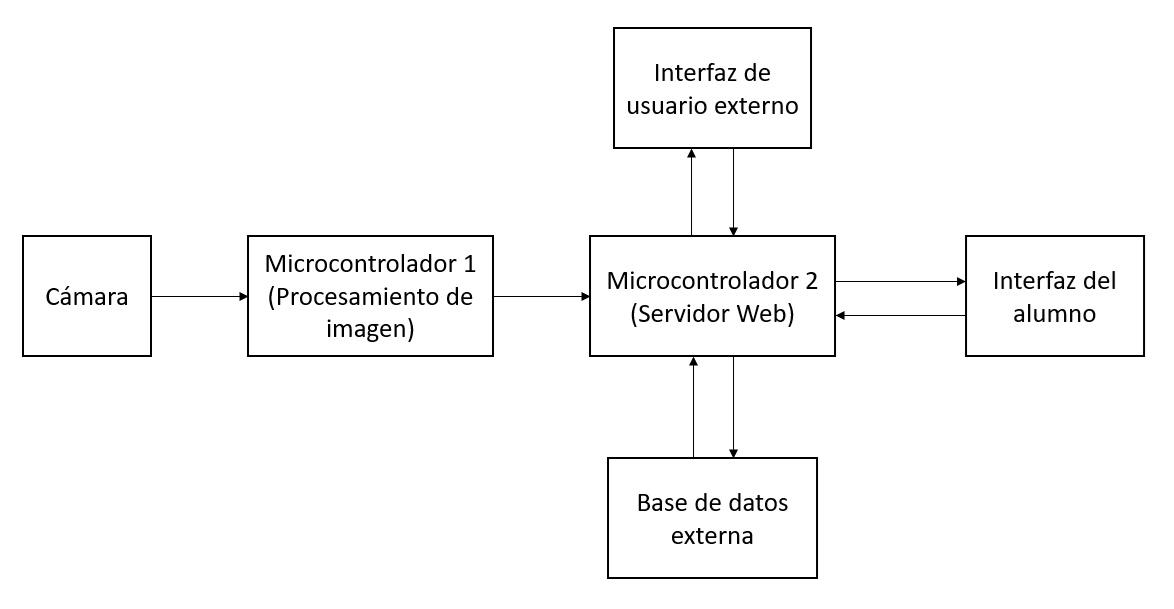
\includegraphics[width=0.3\textwidth]{figuras/bloques2.png}
    \caption{Diagrama de bloques del sistema específico}
    \label{fig:bloques2}
\end{figure}


Utilizando todos estos componentes se logra que este dispositivo sea económico y portable, como se planteó en un inicio. Para además garantizar la ergonomía de uso, todo este sistema irá montado en la visera de una gorra común, para que la cámara pueda tener un buen ángulo del ojo a la vez de que se procura dar un uso cómodo y seguro.

\keyword{(Imagen del montaje teórico?)}


\end{itemize}

\subsection{Tecnologías a utilizar}

En esta sección se listan y justifican todos los componentes de hardware elegidos para este proyecto. Asimismo, se detalla también el rol que cumplirá cada uno en el sistema expuesto en la sección anterior.

\keyword{Microcontroladores}

Los microcontroladores son el eje central del presente trabajo. Estos son los responsables de realizar la captura y procesamiento de imágenes, así como de la ejecución de la aplicación que el usuario final visualizará en su monitor. Como se ha mencionado varias veces a lo largo de este informe, se busca desarrollar un dispositivo económico, por lo que los microcontroladores seleccionados deben ser de bajo costo y fácilmente accesibles. Además, se estableció que el microcontrolador que se utilizará para ejecutar la aplicación web debía poseer alguna forma de conexión WiFi.

En el mercado existen diversos modelos de procesadores que encajan con la descripción buscada, sin embargo, se optó por utilizar los módulos \emph{ESP32-S3}, fabricados por la empresa china \emph{Espressif Systems}.

La figura \ref{fig:familiaesp} muestra un conjunto de placas de desarrollo que utilizan microcontroladores ESP32, mientras que la figura \ref{fig:esp32s3} muestra el microcontrolador \emph{ESP32-S3} seleccionado para este trabajo.

\begin{figure}[htbp]
    \centering
    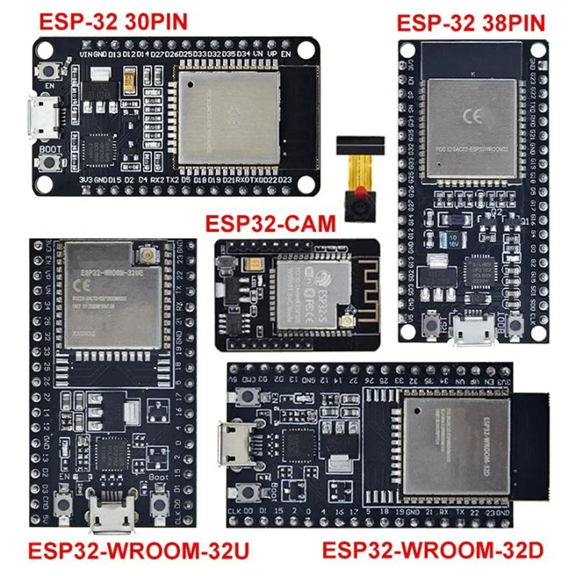
\includegraphics[width=0.3\textwidth]{figuras/familiaesp.png}
    \caption{Algunas placas de desarrollo de la familia ESP32}
    \label{fig:familiaesp}
\end{figure}

\begin{figure}[H]
    \centering
    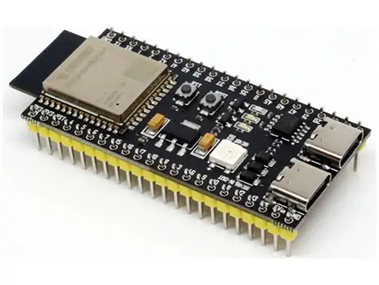
\includegraphics[width=0.3\textwidth]{figuras/esp32s3.png}
    \caption{Placa de desarrollo \emph{ESP32-S3}}
    \label{fig:esp32s3}
\end{figure}

Para establecer un poco el contexto debemos describir sus modelos predecesores, remontándonos al año 2014 cuando salió al mercado el modelo \emph{ESP8266}, una alternativa a las placas Arduino de uso general pero que incluían módulo de WiFi. Había módulos Arduino con WiFi integrado pero no eran económicamente viables, esto último hizo que ganara popularidad rápidamente, por lo que en 2016 llegaría el \emph{ESP-32} estándar, que aunque tenía un precio ligeramente más elevado (~AR\$ 13.000), sus características eran muy superiores al \emph{ESP8266} (Cuenta con más núcleos, más memoria, más periféricos, etc.). Hoy en día tenemos a disposición su variante \emph{ESP32-S3}, el cual es mucho más potente, eficiente, veloz y cuenta con más espacio en memoria RAM que su versión clásica. Si bien su precio suele ser el doble (~AR\$24.000), todas estas características justifican el precio, ya que su potencia será necesaria para correr redes neuronales, transmitir datos y ejecutar aplicaciones web con relativa rapidez.

Cabe recordar que, como se estableció previamente en esta sección, se requiere de dos microcontroladores: uno para capturar y procesar la imagen y otro para servir como punto de acceso WiFi y ejecutar la aplicación web. En ambos casos se utilizará el \emph{ESP32-S3}.
Para capturar las imágenes se requiere una cámara, para lo cual se tiene disponible una placa de desarrollo que utiliza el mismo \emph{ESP32-S3} pero que cuenta con un módulo para insertar cámaras mediante conector flex. 

A continuación se listan algunas placas de desarrollo similares que se tuvieron en consideración y se justifica la razón de su descarte:

\begin{itemize}

\item \emph{ESP8266} y \emph{ESP32} clásico: Como se mencionó anteriormente, se descartan debido a que su memoria y velocidad de procesamiento no son adecuadas para los fines de este proyecto, que incluyen el procesamiento de imágenes y ejecución de redes neuronales.

\item \emph{Raspberry Pi Pico}: Una opción muy sólida, con características técnicas similares o incluso superiores a un \emph{ESP32-S3} y con precios similares. El motivo por el que se descarta es el hecho de no contar con interfaz de cámara nativa, lo que obliga a usar cámaras con circuitos externos complejos, más lentos y que elevan el costo económico del proyecto original. Hay módulos Raspberry Pi que sí incluyen interfaz nativa para cámaras, pero su precio es mayor (>AR\$ 40.000).

\item \emph{Arduino Nano 33 IoT / Arduino Nano ESP32}: Además de contar con las mismas ventajas que el \emph{ESP32-S3}, cuenta con el soporte robusto de la marca Arduino, pero se descarta porque sus costos son más elevados (entre 3 y 5 veces) que los de las placas de Espressif.

\end{itemize}

Además de estas marcas y modelos reconocidos, existen otras placas de desarrollo igual de económicas y eficientes que un \emph{ESP32-S3}, pero estas, a diferencia de las desarrolladas por Espressif, tienen poca disponibilidad en los mercados regionales.

A continuación se listan las características técnicas de los \emph{ESP32-S3}, los microcontroladores elegidos para este trabajo:

\begin{itemize}
\item CPU: Xtensa dual-core 32-bit LX7 DE HASTA 240 MHz

\item Memoria: 384 KB ROM, 512 KB SRAM, 16 KB RTC SRAM 

\item GPIO: 45

\item ADC: 2 × 12-bit SAR ADCs, hasta 20 canales 

\item WIFI AB: 20 MHz, 40 MHz in 2.4 GHz band

\item Bluetooth 5 

\item Interfaces: 3 UART, 4 SPI, 2 I2C, 2 I2S, 1 RMT TX/RX 
\item Contadores y Timers: 1 Contador de pulsos, 3 Watchdog, 4 × 54-bit general, 1 × 52-bit sistema.
\item PWM y USB: LED PWM hasta 8 canales, 2 MCPWM, 1 USB OTG, 1 USB Serial/JTAG

\end{itemize}

\keyword{Cámara}

Existen varios modelos de cámaras compatibles con la interfaz del \emph{ESP32-S3}. Para el procesamiento de imágenes en redes neuronales ligeras no se requiere una cámara de alta resolución, ya que el exceso de datos puede saturar la memoria del microcontrolador. Lo que se debe considerar son dos factores importantes: en primer lugar, la necesidad de una alta tasa de fotogramas por segundo (FPS). Esta velocidad es fundamental, ya que el sistema realiza un rastreo de coordenadas en tiempo real directamente desde el flujo de datos del sensor, en lugar de analizar imágenes estáticas. Por otro lado, al estar el dispositivo montado en la visera de una gorra, el campo de visión (FOV) no debe ser muy amplio, para evitar entorpecer a la red neuronal con estímulos ajenos a la pupila del ojo. Mediante el análisis empírico de imágenes con distintos ángulos, se determinó que para esta tarea es necesario un campo de visión de entre 60 y 120 grados. 

En ese sentido, las cámaras \emph{OV2640} de 2 Megapíxeles (frecuentemente incluídas en la compra de los propios módulos ESP) son una opción adecuada. Sin embargo, existen otros modelos de cámara que también hubieran sido opciones viables, como la \emph{OV3660} de 3 Megapíxeles, que proporciona resultados similares. Debido a su reducida resolución, a la sencillez de adquisición y a que su lente posee un ángulo de visión de 68°, se decidió finalmente implementar la \emph{OV2640} (Figura \ref{fig:ov2640}). Cabe mencionar que existen en su versión acortada o alargada. En este trabajo optamos por la segunda, ya que su flexibilidad ayudará al posterior montaje en la gorra.

\begin{figure}[htbp]
    \centering
    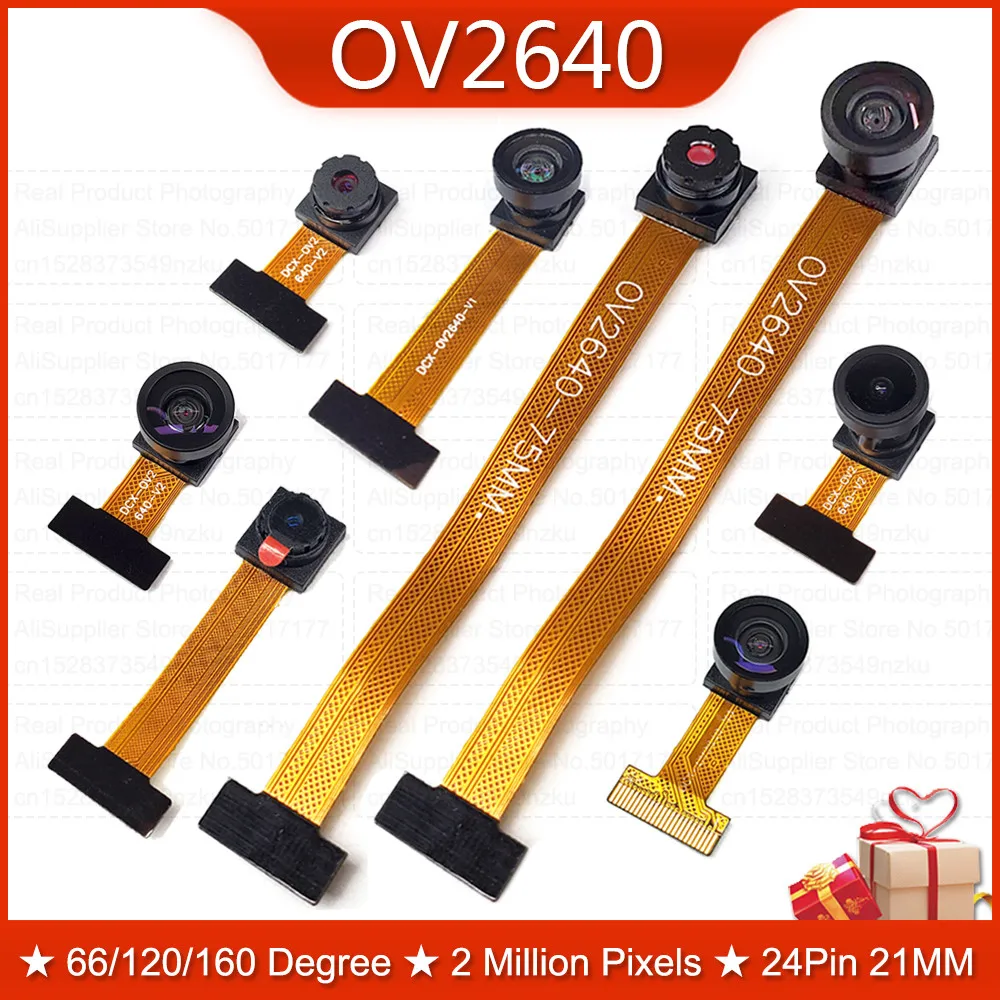
\includegraphics[width=0.3\textwidth]{figuras/ov2640.png}
    \caption{Cámara \emph{OV2640} en distintas formas y ángulos de visión}
    \label{fig:ov2640}
\end{figure}




\keyword{Protocolos de comunicación}

El sistema principal de este dispositivo tiene múltiples componentes operando a la vez y cumpliendo distintas funciones, por lo que es necesario establecer sistemas de comunicación convenientes para garantizar que los datos se transmitan de la manera más segura, rápida y eficiente posible sin comprometer la información y el pleno funcionamiento del prototipo final.

Como se advirtió previamente, el hardware del sistema se estructura en tres bloques fundamentales:

\begin{itemize}

\item Un microcontrolador encargado de capturar y procesar la imagen.

\item Un microcontrolador encargado de interconectar el sistema de captura y procesamiento con la interfaz de usuario.

\item Un dispositivo externo que aloje la interfaz de usuario y muestre de forma didáctica e intuitiva la información.

\end{itemize}

Bajo esta arquitectura, se establecen dos canales de comunicación principales. El primero de ellos vincula a ambos microcontroladores y el segundo enlaza al microcontrolador secundario con el dispositivo externo. 

Respecto al primer enlace, cabe aclarar que no se transmiten los fotogramas del video, sino únicamente los resultados del procesamiento del detector ocular: las coordenadas espaciales (\emph{X} e \emph{Y}) de la pupila y un valor booleano que indica si el ojo se encuentra abierto o cerrado. Como el sistema debe operar en tiempo real, esta transmisión exige alta velocidad y estricta seguridad para evitar la pérdida de paquetes. Para satisfacer estos requisitos, sumado a factores de practicidad física en el diseño, se determinó inicialmente la implementación del protocolo cableado \emph{SPI} (Serial Peripheral Interface). 

El protocolo SPI es un estándar de comunicación de datos en serie normalmente utilizado para comunicar un microcontrolador llamado \emph{maestro} con otro llamado \emph{esclavo} (puede haber uno o varios de cada categoría). Esta forma de comunicación es ideal debido a que es:

\begin{itemize}

\item Sincrónica: Ambas partes están sincronizadas con una misma señal de clock a la hora de comunicarse, lo que garantiza que ningún dato se pierda en el proceso.

\item De baja latencia: A diferencia de otros protocolos, como \emph{UART}, el protocolo SPI es capaz de operar a frecuencias significativamente altas (del orden de los Megahertz) sin perder estabilidad.

\end{itemize}

Estas dos ventajas satisfacen los requisitos de velocidad y seguridad necesarios para la transmisión de las coordenadas de la pupila. En la figura \ref{fig:protocolospi} se ilustra este protocolo de comunicación.

\begin{figure}[htbp]
    \centering
    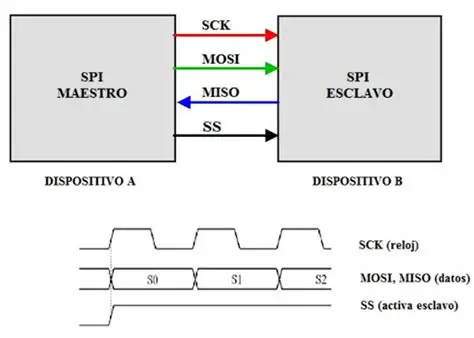
\includegraphics[width=0.5\textwidth]{figuras/protocolospi.png}
    \caption{Funcionamiento del protocolo SPI}
    \label{fig:protocolospi}
\end{figure}

Analizando la comunicación entre el microcontrolador que ejecuta la aplicación web y el dispositivo periférico que muestra la interfaz de usuario, se descarta de entrada un canal de transmisión por cable, ya que el receptor no necesariamente tendrá las mismas características entre una sesión y otra: puede tratarse de una laptop, un celular, una tablet o una computadora de escritorio, y resulta complicado estandarizar un medio físico para todos ellos, además de que se prioriza la comodidad del usuario. Es por eso que se opta por un canal de transmisión inalámbrico, para lo cual se analizaron tres posibilidades detalladas en la tabla \ref{tab:com_inalambrica}


\begin{table}[htbp]
    \centering
    \caption{Sistemas de comunicación inalámbrica}
    \label{tab:com_inalambrica}
    
    \begin{tabular}{|l|>{\raggedright\arraybackslash}p{4cm}|>{\raggedright\arraybackslash}p{4cm}|>{\raggedright\arraybackslash}p{4cm}|}
        \hline
        \textbf{} & \textbf{Bluetooth} & \textbf{Wi-Fi} & \textbf{RadioFrecuencias} \\
        \hline
        \textbf{Alcance} & Bajo (unos pocos cm) & Medio (varios metros) & Muy alto (Kilómetros)\\
        \hline
        \textbf{Accesibilidad de hardware} & La gran mayoría de dispositivos soporta Bluetooth & Prácticamente todos los dispositivos soportan Wi-Fi y tienen un navegador instalado & Generalmente requieren hardware externo para leer radiofrecuencias\\
        \hline
        \textbf{Accesibilidad de Software} & Se requiere una app nativa para interpretar los datos & Soporta protocolo TCP-IP & Se requiere una app nativa para interpretar los datos\\
        \hline
    \end{tabular}
    
\end{table}

Por todos los motivos anteriormente evaluados, se opta por utilizar conexión Wi-Fi.

\keyword{Entornos de desarrollo}

La programación del hardware requiere la utilización de un Entorno de Desarrollo Integrado (IDE) para escribir, compilar y cargar el código en la placa de desarrollo. Para este proyecto se optó por el software \emph{Visual Studio Code} junto con la extensión \emph{PlatformIO}, ya que la eficiencia en la gestión de dependencias y librerías facilita el trabajo con una amplia variedad de microcontroladores.
Adicionalmente, se realizaron pruebas utilizando \emph{Arduino IDE}. Dado que los microcontroladores de la familia ESP32 son compatibles con las librerías de Arduino, esta alternativa permitió una evaluación más ágil del microcontrolador durante las etapas iniciales de desarrollo en comparación con el entorno oficial provisto por \emph{Espressif} (\emph{ESP-IDF}).
Por otra parte, para la etapa de experimentación y entrenamiento de los modelos matemáticos de redes neuronales orientados a la detección ocular, se utilizó el entorno basado en la nube \emph{Google Colab}, el cual permite la ejecución de código Python en notebooks interactivos.

\begin{figure}[htbp]
    \centering
    
\includegraphics[width=0.5\textwidth]{figuras/entornos.png}
    \caption{Entornos de desarrollo (\emph{Visual Studio Code, PlatformIO, Arduino IDE y Google Colab})}
    \label{fig:entornos}
\end{figure}

\section{El detector ocular}

En esta sección se describe el desarrollo del sistema de detección ocular, el cual experimentó múltiples modificaciones e iteraciones hasta llegar al resultado final.

\subsection{Procesamiento local}

En un principio se estableció que el procesamiento de imágenes se realizaría en una de las placas \emph{ESP32-S3} mediante una red neuronal artificial de tipo convolucional. Al ser el propio microcontrolador el encargado de gestionar todas estas tareas de detección es que se habla de \keyword{procesamiento local}. 
Lograr que un microcontrolador ejecute una red neuronal de detección de ese calibre no es tarea sencilla, puesto que la mayoría de estos modelos exigen una alta capacidad de memoria y velocidad que suele exceder a lo que el \emph{ESP32-S3} puede ofrecer. Es por esto que se comenzó a explorar formas de diseñar y entrenar redes neuronales lo más livianas y sencillas posibles.
A este paradigma de trabajo que busca la implementación de inteligencia artificial con recursos y software y hardware limitados se lo conoce como \keyword{Tiny Machine Learning} (o \keyword{TinyML}), y es la filosofía que se aplicó en el desarrollo de este dispositivo.

\keyword{Edge Impulse}

Un primer acercamiento a la disciplina del \emph{Tiny Machine Learning} puede darse con el uso de \emph{Edge Impulse}, una plataforma de desarrollo basada en la nube orientada específicamente al aprendizaje automático con bajos recursos computacionales (Figura \ref{fig:edgeimpulse}). Fundado en 2019 con el objetivo de facilitar esta tarea, su principal función es trasladar el procesamiento desde servidores en la nube directamente al hardware local. Es una plataforma muy versátil, ya que ofrece compatibilidad con los entornos de desarrollo previamente mencionados y con el framework de Arduino. 

\begin{figure}[htbp]
    \centering
    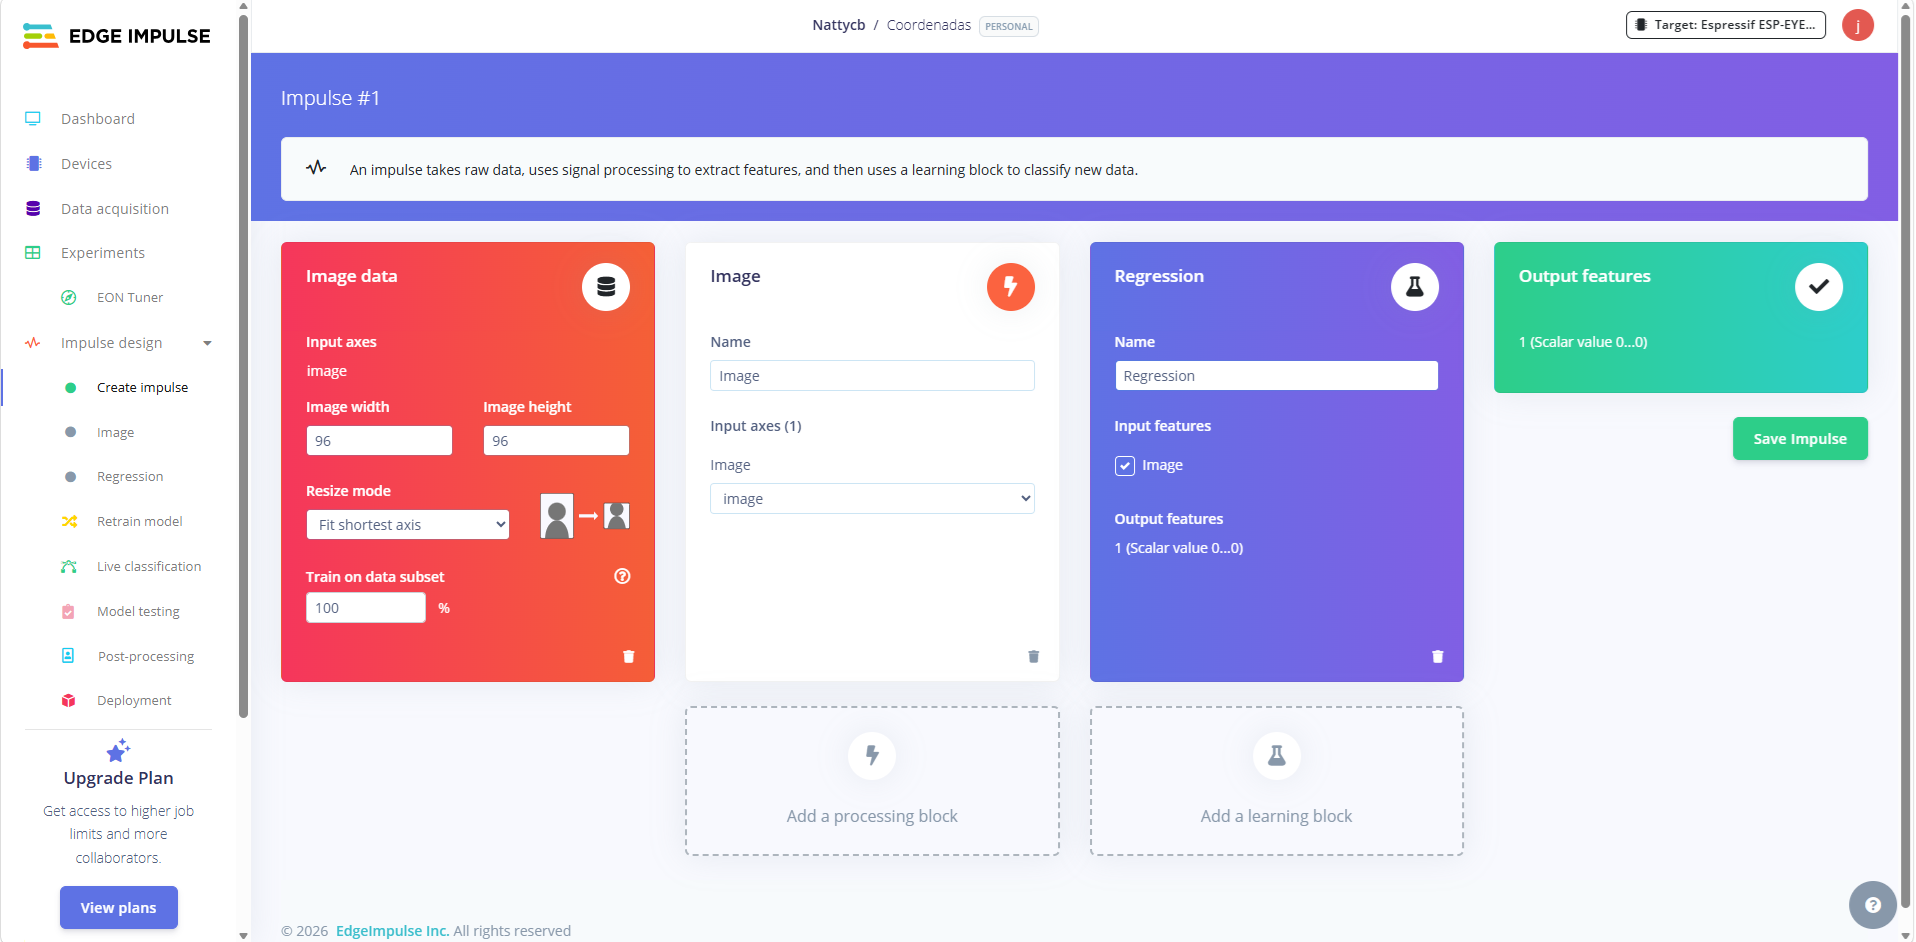
\includegraphics[width=0.3\textwidth]{figuras/edgeimpulse.png}
    \caption{Pantalla de creación de modelos de \emph{Edge Impulse}}
    \label{fig:edgeimpulse}
\end{figure}

Su funcionamiento se basa en una estructura de trabajo lineal (conocido como \emph{pipeline} o \emph{Impulse}). Este flujo unifica todas las etapas del desarrollo de un modelo predictivo: comienza con la adquisición y etiquetado de datos estructurados, continúa con bloques de procesamiento digital de señales (para extraer las características más relevantes de imágenes o audio), sigue con el entrenamiento de la red neuronal propiamente dicha y finaliza con el empaquetado del modelo. Todo esto mediante una interfaz de usuario intuitiva.

Con las técnicas de cuantización que realiza y sus métodos de aceleración de hardware, resulta una opción prometedora que optimiza todo el proceso de aprendizaje. Funciona muy bien para tareas sencillas como reconocimiento de objetos o rostros (Figura \ref{fig:deteccionverduras}).

\begin{figure}[htbp]
    \centering
    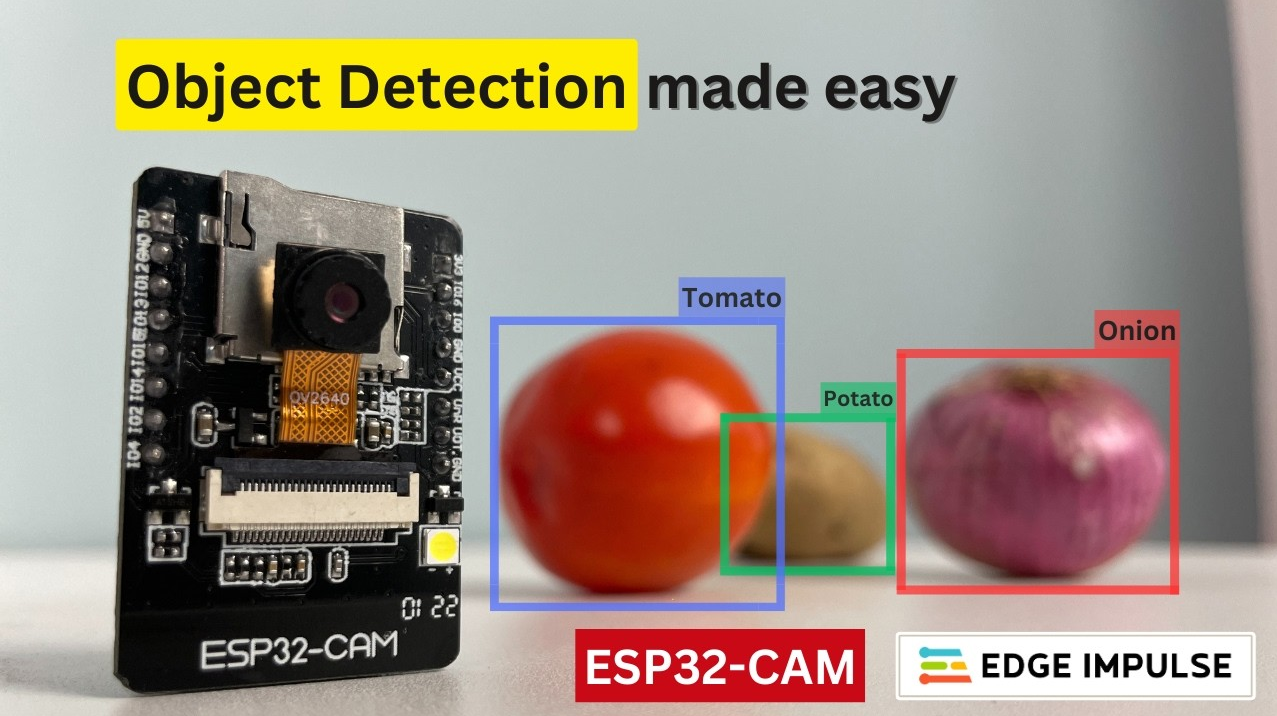
\includegraphics[width=0.5\textwidth]{figuras/deteccionverduras.png}
    \caption{Reconocimiento de vegetales con \emph{EdgeImpulse}}
    \label{fig:deteccionverduras}
\end{figure}

Sin embargo, tras varias pruebas realizadas con datasets (conjunto de datos de entrada conocidos) sencillos, se determinó que este método no alcanzaba la precisión requerida para la detección continua de coordenadas espaciales a tiempo real, o siquiera para determinar hacia qué dirección se dirigía la mirada (arriba, abajo, izquierda o derecha).

Además, al momento de cargar la red exportada en el procesador \emph{ESP32}, el monitor serial evidenció que cada inferencia demoraba entre 700 y 1000 milisegundos en finalizar, una latencia sumamente indeseable cuando se busca un seguimiento en tiempo real.

Debido a estas imprecisiones y demoras se decidió descartar esta solución.

\keyword{(Imágenes de la imprecisión o el delay)}



\keyword{TensorFlow Lite}

Una herramienta muy utilizada en Machine Learning es el framework de código abierto \emph{TensorFlow (TF)}, el cual está diseñado para entrenar y ejecutar modelos de redes neuronales propias o ya existentes. El principal problema radica en que este entorno no está optimizado para ejecutar estas redes en sistemas con hardware limitado como lo es el microcontrolador \emph{ESP32}, y es por eso que Google desarrolló una versión más liviana dedicada a facilitar este tipo de situaciones, llamada \emph{TensorFlow Lite (TFLite)}, junto con su variante específica para arquitecturas sin sistema operativo: \emph{TensorFlow Lite for Microcontrollers (TFLM)}. 

Como primera instancia, se pensó para este trabajo desarrollar un modelo propio con datos de entrada tomados por la propia \emph{ESP32} y mantener un control absoluto de la optimización y exportación del modelo. Esto último es una enorme ventaja que se tiene respecto al uso de \emph{Edge Impulse}, ya que permite gestionar exactamente cómo se comprime la red para el microcontrolador, evitando las limitaciones y la sobrecarga de código de una plataforma cerrada. 

Para facilitar el proceso de creación del modelo, Google ofrece también la herramienta \emph{Keras}, una API de alto nivel que agiliza y simplifica enormemente la programación de la arquitectura neuronal. Es por esto que el entorno de desarrollo seleccionado para esta tarea fue \emph{Google Colab} (Figura \ref{fig:entornogooglecolab}) utilizando el lenguaje Python.

\begin{figure}[htbp]
    \centering
    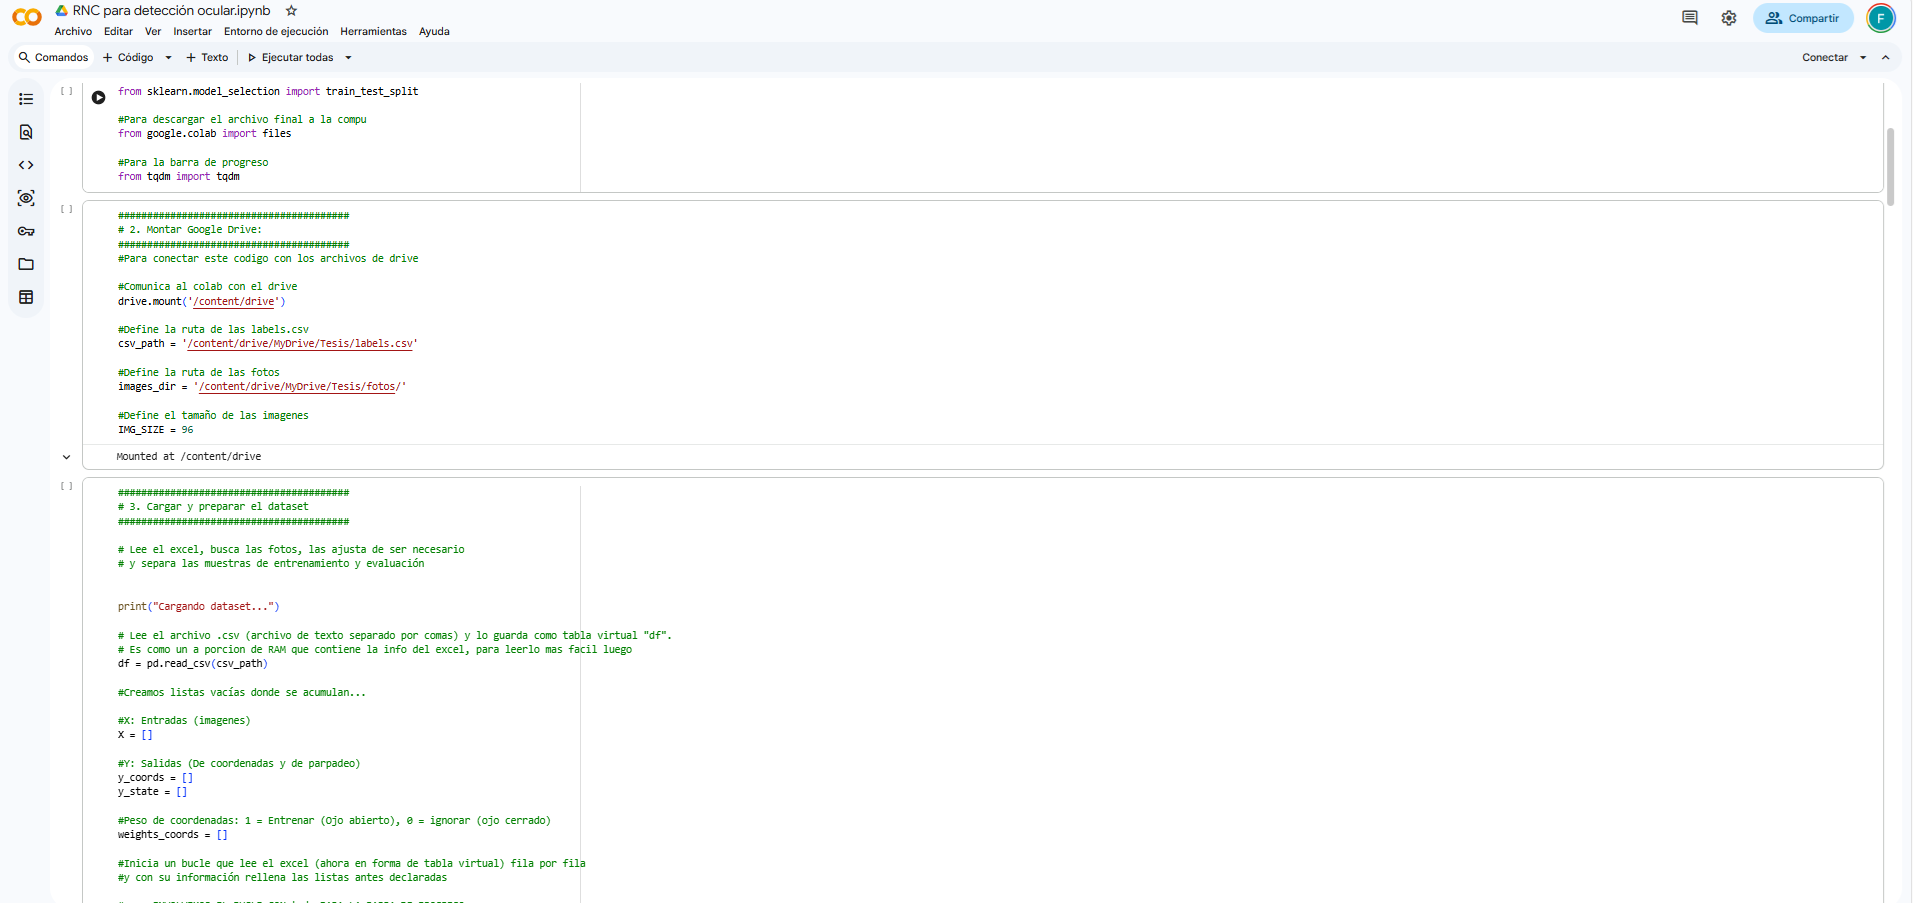
\includegraphics[width=0.3\textwidth]{figuras/entornogooglecolab.png}
    \caption{Entorno de \emph{Google Colab}}
    \label{fig:entornogooglecolab}
\end{figure}

Antes de empezar a codificar es necesario un \emph{dataset}. Para una red de este tipo, normalmente se utilizan cientos de imágenes asociadas a lo que se denominan \emph{etiquetas}. Una etiqueta representa el valor objetivo que el modelo debe predecir y aprender. Para este proyecto, las etiquetas corresponden a números enteros fijos que representan las coordenadas espaciales (\emph{X} e \emph{Y}) del centro de la pupila. 

Las imágenes de entrenamiento fueron capturadas utilizando el módulo \emph{ESP32-CAM} en formato de escala de grises (\emph{Grayscale}) y con una resolución de 96x96 píxeles. Esta configuración se seleccionó con el propósito de minimizar el consumo de recursos computacionales sin comprometer los detalles necesarios en la imagen. Para garantizar cantidad y variabilidad en los datos, se tomó un conjunto total de 1315 capturas obtenidas de cinco personas distintas, contemplando distintas condiciones de iluminación y variaciones físicas como la presencia y ausencia de anteojos.

\keyword{(Imágenes de algunas de las 1315 fotos)}

En paralelo, las coordenadas correspondientes a cada imagen (expresadas en pixeles dentro de una imagen 96x96), se anotaron en una hoja de cálculo, estructurando así los datos para su posterior utilización en el entrenamiento.

\begin{figure}[htbp]
    \centering
    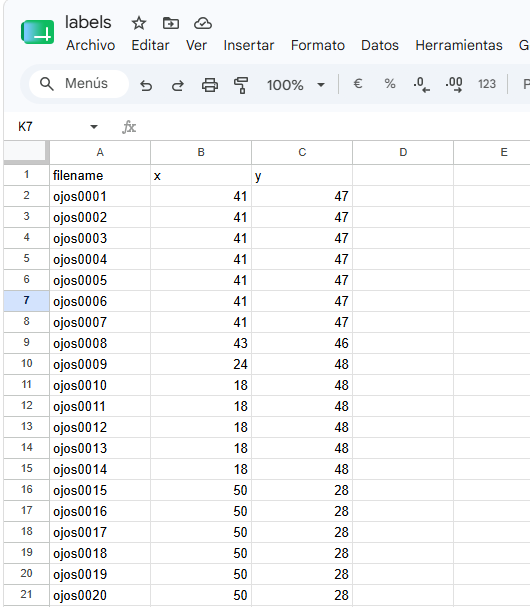
\includegraphics[width=0.5\textwidth]{figuras/etiquetas.png}
    \caption{Planilla con etiquetado de imágenes}
    \label{fig:etiquetas}
\end{figure}

A continuación se listan y explican brevemente las etapas de la creación del modelo de la Red Neuronal Convolucional (CNN) en \emph{Google Colab} con \emph{Python/Keras}:

\begin{enumerate}

\item Preparación: Se comienza importando en el código las herramientas necesarias para construir la CNN. Entre ellas \emph{Tensorflow}, \emph{Pandas}, \emph{Numpy}, \emph{OpenCV}, entre otros. Se monta la herramienta de \emph{Google Drive}, para que el entorno pueda acceder a las imágenes y etiquetas almacenadas allí.

\item Formateo del dataset: Se extraen de \emph{Google Drive} las 1315 imágenes, se las recorta a 96x96 de ser necesario y se leen y almacenan las etiquetas en arreglos.

\item Creación de la red: Se crea el modelo indicando el formato de sus entradas, sus capas internas y su función de activación. Al final se compila el modelo indicando cómo trabajará con los errores.

\item Separación de datos: Aquí se aplica una técnica para entrenar y evaluar la red al mismo tiempo. Se separan las imágenes del dataset en dos grupos: el grupo de entrenamiento (un 80\% de las imágenes) y el grupo de evaluación (el 20\% restante). Esta separación es aleatoria y sirve para comprobar el resultado de la construcción del modelo.

\item Entrenamiento: Se realiza el entrenamiento en sí mismo eligiendo el número de \emph{épocas} (veces que el modelo analiza el grupo de imágenes) y aplicando \emph{callbacks} (funciones que detienen el entrenamiento cuando se alcanza la precisión deseada), para evitar que la red memorice fotos en lugar de aprender de ellas.

\item Evaluaciones: Se pone a prueba la red insertándole la porción de datos que nunca vió durante su entrenamiento. Se muestran los resultados y análisis de distintos parámetros estadísticos como el porcentaje de aciertos, los errores, la muestra con peor desviación, etc.

\item Exportación: Se exporta el modelo a un archivo en formato \emph{.tflite} para ser utilizado en el entorno de \emph{Visual Studio Code}.

\end{enumerate}

Tras iterar sobre la arquitectura de la red y ajustar sus hiperparámetros, tales como la cantidad de capas y los filtros de procesamiento, para maximizar la precisión (Figura \ref{fig:resultadoscolab}), se procedió a exportar el modelo y compilarlo en el entorno de C++ para evaluar su rendimiento en vivo.  

\begin{figure}[htbp]
    \centering
    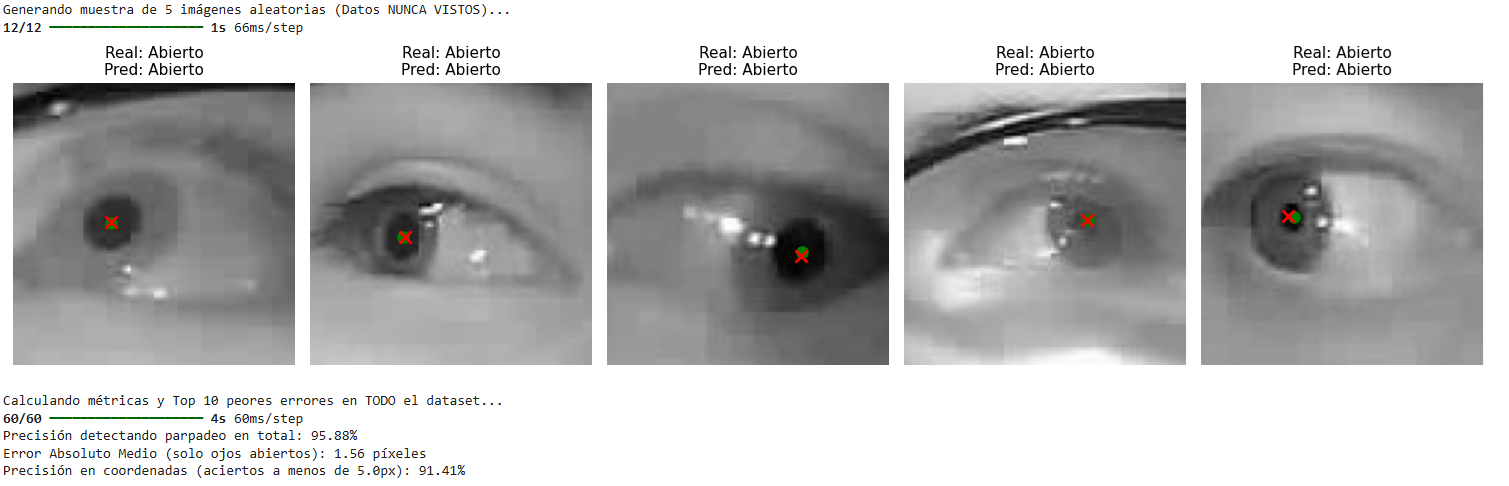
\includegraphics[width=0.5\textwidth]{figuras/resultadoscolab.png}
    \caption{Resultados del modelo desarrollado en \emph{Google Colab}}
    \label{fig:resultadoscolab}
\end{figure}

Si bien este modelo demostró ser significativamente más rápido, eficiente y controlable que la opción generada mediante \emph{Edge Impulse}, las pruebas empíricas en tiempo real mostraron que no cumplía con los requisitos de precisión para ser utilizado en el dispositivo final. Al operar el sistema, el modelo presentaba una alta inestabilidad en las predicciones: el cursor de la interfaz sufría de oscilaciones pequeñas y constantes (\emph{jittering}) y era incapaz de mantener una posición firme o realizar un seguimiento fluido de la mirada.

\keyword{(Imagenes de las fallas)}

Al intentar reducir esa inestabilidad, se encontró un límite de hardware insalvable: aumentar la complejidad y profundidad de la red neuronal para estabilizar la predicción disparaba la latencia de procesamiento a niveles inaceptables, mientras que simplificar la arquitectura para recuperar velocidad degradaba la exactitud de las coordenadas.

\keyword{(Imagenes del monitor serial con los delays)}

A partir de este compromiso insuperable entre latencia y precisión, se concluye que el procesamiento neuronal de imágenes de forma puramente local dentro de las limitaciones de memoria del microcontrolador no resulta viable para las exigencias de este proyecto. Esta limitación motiva el descarte definitivo en el uso de redes neuronales en hardware de bajos recursos. Sin embargo, para mantener el enfoque de este trabajo, no se sustituirá el hardware base, sino que se buscará otro método con un procesamiento más sencillo.

\keyword{Detección por umbral de oscuridad y brillantez}

Al no tener éxito en el procesamiento de imágenes mediante el uso de redes neuronales convolucionales, se optó por un método de visión computacional clásica. Este consiste en capturar constantemente una imagen en escala de grises y analizar en tiempo real sus patrones de oscuridad (intensidad lumínica).

Cuando se toma una imagen del ojo de un individuo, en la inmensa mayoría de los casos el punto más oscuro resulta ser la pupila (Figura \ref{fig:oscuridadpupila}), puesto que el resto de la imagen está compuesto por porciones irregulares de distintos tonos grises más claros. Este método aprovecha esa oscuridad extrema para señalar con un cursor la ubicación exacta de la pupila, y por lo tanto inferir la dirección de la mirada.

\begin{figure}[htbp]
    \centering
    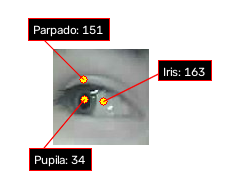
\includegraphics[width=0.9\textwidth]{figuras/oscuridadpupila.png}
    \caption{Distintas partes del ojo y su nivel de oscuridad}
    \label{fig:oscuridadpupila}
\end{figure}

Para entender este método se debe aclarar previamente el funcionamiento del procesamiento de imágenes en el microcontrolador. Al capturar un fotograma, el \emph{ESP32} lo almacena en un \emph{framebuffer}, es decir, un bloque de memoria reservado estructurado como una matriz bidimensional. Si se trabaja en escala de grises, cada elemento de esta matriz contiene un número entero comprendido entre 0 y 255. Este valor representa la intensidad lumínica del píxel en esa posición espacial específica (donde 0 equivale a oscuridad absoluta y 255 a saturación blanca). 

El algoritmo procesa la imagen realizando un barrido inicial revisando cada píxel para identificar el valor de intensidad mínimo (el punto más oscuro del fotograma). Para evitar que la detección dependa de un único píxel, lo cual arriesgaría la estabilidad, se establece un umbral de oscuridad dinámico. Esto significa que el algoritmo no aísla solamente el píxel más oscuro, sino a toda una región de píxeles cuyos valores de intensidad se encuentren por debajo de dicho umbral. 

Una vez seleccionada la región de interés (\emph{ROI}) que teóricamente abarca a la pupila, el programa ejecuta un segundo barrido para calcular sus coordenadas centrales mediante la aplicación de un centroide ponderado. A diferencia de un promedio simple, donde se suman todas las coordenadas y se dividen por la cantidad de píxeles detectados, el centroide ponderado asigna un factor de peso a cada coordenada en función de su nivel de oscuridad.
Mientras más oscuro sea un píxel, mayor será su peso matemático en la ecuación final. Esta ponderación resulta fundamental para la estabilidad del sistema, ya que otorga una influencia dominante al núcleo de la pupila (altamente oscura) y reduce considerablemente las desviaciones causadas por sombras periféricas o pestañas que hayan ingresado dentro del umbral de detección (grises más claros).

\keyword{(Imagen del cálculo con centroide en el código)}

Este algoritmo, mucho más liviano que una red neuronal convolucional, redujo considerablemente el tiempo de procesamiento y aumentó la eficiencia de recursos de memoria en el \emph{ESP32}. Sin embargo, presentaba un problema importante: la iluminación ambiental.
Al evaluar este método se descubrió que su precisión dependía exclusivamente de la luminosidad de la imagen. Un ambiente con mucha luz genera sombras pronunciadas que el algoritmo puede confundir con las pupilas. Por el contrario, en un ambiente con poca luz, el nivel de oscuridad de la pupila y de otras áreas (como pestañas o cejas) se vuelve demasiado similar. A pesar de que el umbral de oscuridad puede ajustarse mediante código, resulta poco práctico si se considera que la luz ambiental es una variable incontrolable y sumamente dinámica, motivo por el cual este algoritmo se descarta como una solución óptima para la detección ocular definitiva.

A pesar de que la iluminación ambiental es una variable incontrolable, lo que sí se puede controlar es la iluminación de la imagen captada por el \emph{ESP32}. Si hubiese una fuente de luz junto a la cámara, esta variable sería siempre constante y se evitaría confusiones con sombras o pestañas. Sin embargo, alumbrar el ojo del usuario con luz visible permanentemente sería molesto y un perjuicio para su visión, por lo que se tuvo que plantear un método de iluminación para que solo la cámara del microcontrolador pudiera detectar sin dañar la vista: la luz infrarroja.
La luz infrarroja (IR) tiene longitudes de onda mayores a las de la luz visible, por lo que es indetectable por el ojo humano, mientras que los sensores de las cámaras digitales sí son capaces de captarla. Es por eso que colocar un diodo LED emisor de luz infrarroja junto a la cámara parecía ser la solución perfecta para este problema. Sin embargo, se impuso otro obstáculo físico a superar: el efecto del brillo corneal.

Al ser húmeda y curva, la superficie de la córnea del ojo actúa como un espejo esférico perfecto para estas ondas infrarrojas. La luz rebota en la superficie del ojo generando un punto blanco muy intenso y concentrado (denominado \emph{Glint}). Esto ocasionó errores severos en el algoritmo anterior de detección de oscuridad, por lo que se decidió modificarlo para utilizar este fenómeno físico a favor: en lugar de detectar los píxeles más oscuros, se invirtió la lógica para detectar los píxeles más claros mediante un umbral de brillantez. 

\keyword{(Imagen del glint)}

Lamentablemente, esta solución tampoco resultó viable. Al realizar las pruebas de seguimiento, se comprobó que el glint no se desplaza de la misma forma que la pupila: su posición relativa depende estrictamente de la geometría del ojo frente a la fuente de luz.

\keyword{(Imagen del glint desplazado)}

De este modo, tras exhaustivos análisis, pruebas y cambios de lógica, se demostró que estos algoritmos de detección de oscuridad y brillantez no alcanzaban la precisión requerida para el correcto funcionamiento del dispositivo. En consecuencia, se concluye que el procesamiento de imagen directamente en el microcontrolador no cumple con las expectativas impuestas al inicio de este trabajo, por lo que queda descartado definitivamente.


\subsection{Procesamiento remoto}

Tras las limitaciones comprobadas en la aplicación de métodos de detección ocular utilizando los recursos de un microcontrolador, se optó por prescindir del procesamiento local en el hardware base y derivar esta tarea a un dispositivo externo. Es por ello que los métodos expuestos a continuación se engloban en la categoría de \emph{procesamiento remoto}. En este sentido, el microcontrolador se encarga exclusivamente de capturar las imágenes y alojar la aplicación web, mientras que el procesamiento matemático de los fotogramas es ejecutado por el dispositivo cliente. 
Debido a la reducción considerable de la exigencia al microcontrolador capturador (pues su única tarea es capturar fotogramas y transmitirlos), se optó por ahorrar más recursos utilizando un \emph{ESP32-CAM}, una versión menos potente y más económica que el \emph{ESP32-S3}.

\keyword{Redes neuronales pre-entrenadas}

Al no tener la limitación de la velocidad de procesamiento del microcontrolador, se puede optar por utilizar una red neuronal pre-fabricada más potente para la detección de coordenadas.
Dos alternativas consideradas fueron \emph{MediaPipe} (un conjunto de librerías provisto por Google) y \emph{WebGazer} (un modelo desarrollado en el ámbito académico). Ambas son herramientas basadas en tecnologías web que solucionarían todos los problemas de iluminación ambiental descritos con anterioridad, pero fueron rápidamente descartadas debido a dos inconvenientes.

\begin{figure}[htbp]
    \centering
    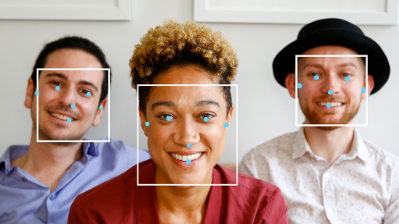
\includegraphics[width=0.5\textwidth]{figuras/deteccion_rostro_mediapipe.png}
    \caption{Detección de rostro con \emph{MediaPipe}}
    \label{fig:deteccion_rostro_mediapipe}
\end{figure}

\begin{figure}[htbp]
    \centering
    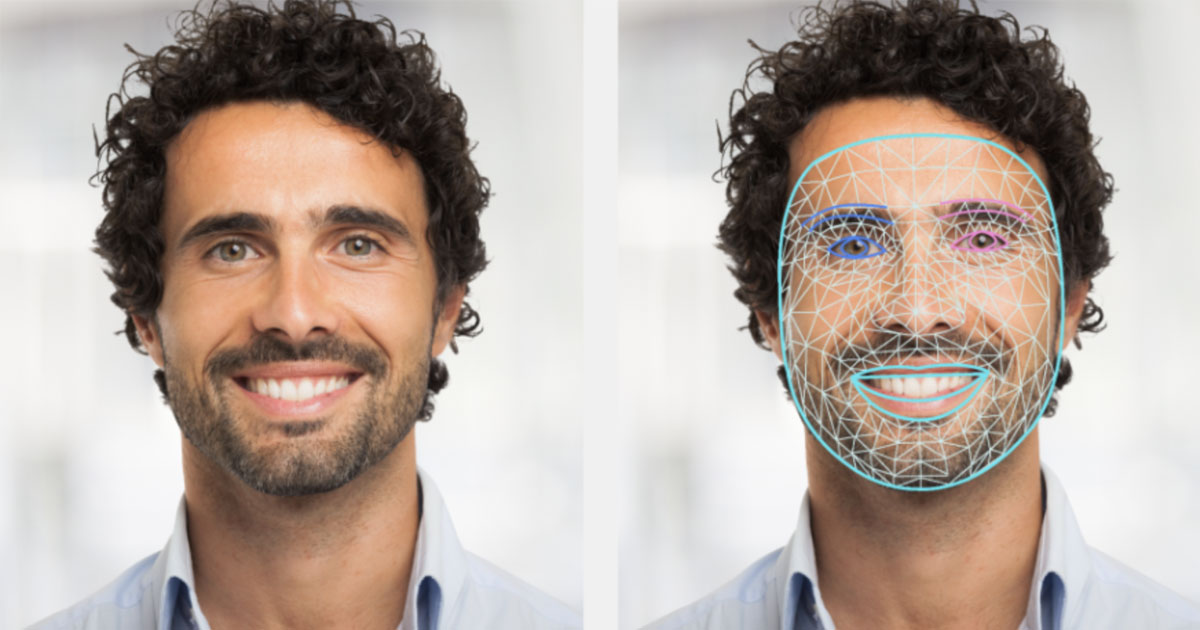
\includegraphics[width=0.5\textwidth]{figuras/seguimiento_rostro_mediapipe.png}
    \caption{Facciones del rostro en \emph{MediaPipe}}
    \label{fig:seguimiento_rostro_mediapipe}
\end{figure}

\begin{figure}[htbp]
    \centering
    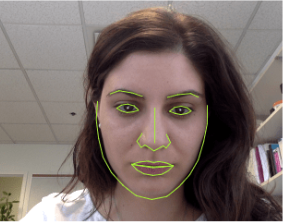
\includegraphics[width=0.7\textwidth]{figuras/deteccion_rostro_webgazer.png}
    \caption{Facciones del rostro en \emph{WebGazer}}
    \label{fig:deteccion_rostro_webgazer}
\end{figure}

Por un lado, ambos son detectores de expresiones faciales y no están diseñados para seguir específicamente el movimiento de la pupila. Si bien los algoritmos se pueden adaptar, requieren una vista completa del rostro para poder anclar sus referencias. Esto implica perder precisión en las coordenadas exactas del ojo (al tener que medir variaciones minúsculas en píxeles) e invalida el diseño físico planeado originalmente para este proyecto (una cámara que capte únicamente la región ocular). 

El otro inconveniente es que estas redes son demandantes en términos del hardware de captura necesario para su ejecución. Utilizar la cámara de baja resolución del \emph{ESP32} de forma focalizada no es la condición ideal para que estos modelos operen con normalidad. Se podría deducir que esto se soluciona derivando la tarea de captura de imagen a las cámaras integradas de los dispositivos externos (PC, celular o tablet), pero esto comprometería una característica vital del dispositivo final: la versatilidad. Cada dispositivo cliente posee una cámara con propiedades distintas, variando drásticamente su resolución, ubicación, distancia focal e inclinación. Todas estas son variables incontrolables que afectarían la precisión del seguimiento espacial, algo que se evita por completo al utilizar un dispositivo que mantiene siempre su propia cámara en una posición fija y calibrada respecto al ojo.
Por todos estos motivos empíricos y de diseño, se decide prescindir definitivamente de las redes neuronales como métodos de detección espacial.

\keyword{OpenCV con circulos de Hough}

La librería \emph{OpenCV} (Open Source Computer Vision Library) es una biblioteca de software de código abierto especializada en visión computacional y procesamiento de imágenes. Su principal ventaja es que está altamente optimizada para aplicaciones en tiempo real. En lugar de tener que escribir desde cero las complejas operaciones matemáticas para leer matrices de píxeles, detectar bordes o filtrar ruido, \emph{OpenCV} ofrece herramientas y funciones prefabricadas que ejecutan estos cálculos aprovechando al máximo la arquitectura del procesador del dispositivo cliente. 

Por todo lo anterior, además de contar con mayor versatilidad que las redes neuronales anteriormente expuestas, \emph{OpenCV} se perfiló como una alternativa sumamente viable para utilizar en este trabajo. La principal desventaja de este método es que desarrollar el detector requiere la creación de una aplicación nativa en Python que cada dispositivo cliente debe instalar y ejecutar por su cuenta. Evaluando ambos aspectos, se optó por aceptar esta dependencia de software en pos de obtener un detector ocular funcional y robusto. 

Para aprovechar al máximo las capacidades de \emph{OpenCV}, se decidió complementarlo con un algoritmo matemático que se conoce como la \emph{Transformada de Hough}. Es un método clásico de extracción de características utilizado en el análisis de imágenes digitales. Su variante para círculos (conocida como \emph{HoughCircles} en \emph{OpenCV}) funciona analizando los bordes detectados en un fotograma mediante un sistema matemático de \emph{votación}. El algoritmo busca conjuntos de píxeles que compartan una curvatura y se encuentren a una distancia constante (el radio) de un posible punto central. Si suficientes píxeles \emph{votan} por el mismo centro, el algoritmo confirma la existencia matemática de un círculo en esa región. En este contexto, el círculo vendría a ser el iris del ojo, y para determinar las coordenadas exactas de la pupila simplemente se debe calcular la ubicación del centro de dicho círculo.

Para lograr esto, en primer lugar se debe transferir la imagen desde el microcontrolador capturador hacia el dispositivo cliente, para lo cual se opta por utilizar una conexión Wi-Fi mediante protocolo \emph{UDP}. Se descarta la transmisión SPI puesto que no es adecuada para manejar el alto ancho de banda que requiere la transmisión fluida de imágenes. Una vez logrado esto (proceso que se detalla posteriormente en este informe), empieza el trabajo del procesador (CPU) del dispositivo cliente.

Ya recibido el fotograma, \emph{OpenCV} realiza un proceso de filtrado espacial (preprocesamiento) para limpiar la imagen de ruido digital y prepararla para el análisis. A continuación, se le aplica la función de círculos de Hough, y en el momento en el que se detecta el contorno del iris se grafican los resultados sobre la imagen a modo de depuración visual: un trazo verde delimitando la circunferencia detectada, con un punto rojo en su centro que representa las coordenadas de la pupila. 

\keyword{(Imagen de este método funcionando)}

Aquí surge un problema importante. La función de círculos de Hough está matemáticamente diseñada para detectar circunferencias perfectas, y el iris humano no siempre se presenta como tal frente a la cámara: frecuentemente, los párpados ocluyen una parte superior o inferior, alterando así su geometría circular. Esto implicaría que el usuario debería forzar permanentemente sus músculos oculares para mantener los ojos abiertos de forma antinatural y garantizar el correcto funcionamiento del sistema, lo cual resulta poco práctico y sumamente indeseable. 

\keyword{(Imagen con párpados semicerrados)}

Una posible solución consiste en disminuir la exigencia de \emph{OpenCV} para que no detecte únicamente círculos perfectos, sino que tenga cierta tolerancia ante las deformaciones (permitiendo la detección de arcos incompletos o formas elípticas). Esto, sin embargo, genera un problema secundario grave, puesto que el algoritmo se vuelve demasiado permisivo y comienza a registrar falsos positivos al detectar curvas en párpados, cejas, arrugas y otras facciones del rostro. 

\keyword{(Imagen de falsos positivos)}

Ambos problemas presentan un compromiso técnico recíproco, debido a que si se intenta reducir uno, el otro empeora. Luego de sucesivas pruebas utilizando herramientas complementarias como umbrales de radio y detectores de brillantez/oscuridad apoyados por el LED infrarrojo, se concluye que la precisión alcanzada no es la adecuada para un seguidor ocular en tiempo real, por lo que esta solución queda definitivamente descartada.
De esta forma, tras varios intentos insatisfactorios, se toma una decisión radical en el desarrollo de este trabajo: dejar atrás la detección de coordenadas espaciales específicas y pasar a identificar patrones de orientación de la mirada.


\emph{Detección de similaridad estadística}

Este método busca simplificar el sistema de detección ocular con el fin de disminuir la carga de procesamiento, a la vez que elimina toda posible causa de errores tratada con anterioridad. El objetivo es lograr un algoritmo independiente de la luz ambiental, de la resolución de la cámara y de las variaciones en las formas geométricas biológicas del ojo. 

Para evitar, a su vez, la dependencia de aplicaciones nativas de Python, se optó por implementar este algoritmo directamente en una aplicación web. Esta interfaz se aloja en la memoria del propio \emph{ESP32} servidor, y es transmitida al dispositivo cliente externo. Esto implica que el usuario simplemente debe conectarse a la red Wi-Fi generada por el microcontrolador y abrir su navegador de preferencia para poder utilizar el sistema.  Los detalles del desarrollo de esta aplicación se exponen posteriormente en este informe.

\emph{(Diagrama de bloques del nuevo sistema)}

Este sistema de detección requiere, como paso inicial, un proceso de calibración. Para ello, se captura un número definido de imágenes de referencia que representarán todas las acciones posibles dentro de la interfaz. Para garantizar la máxima estabilidad y mitigar posibles confusiones en el algoritmo, se optó por limitar estas acciones a seis:

\begin{itemize}

\item Mirada hacia arriba a la izquierda (Seleccionar opción 1)

\item Mirada hacia arriba a la derecha (Seleccionar opción 2)

\item Mirada hacia abajo a la izquierda (Seleccionar opción 3)

\item Mirada hacia abajo a la derecha (Seleccionar opción 4)

\item Mirada hacia el centro de la pantalla (Zona neutra, no realiza ninguna acción)

\item Parpadeo (Confirmar opción elegida)

\end{itemize}

\emph{(Imagen de los seis moldes)}

Una vez capturadas estas seis imágenes (con resolución 96x96 en escala de grises), se almacenan temporalmente en la memoria del navegador para tenerlas a disposición como plantillas durante la posterior ejecución. Con el sistema en marcha, el \emph{ESP32} captura el ojo en tiempo real con una resolución nativa de 320x240 píxeles en formato de color estándar y envía los fotogramas al navegador web mediante la red local.  Es allí, aprovechando los recursos del dispositivo cliente, donde se produce el procesamiento comparativo de las imágenes. 

\emph{(Imágenes del stream)}

Se comienza con un previo ajuste de la imagen a procesar, esto es, recortar la imagen a un tamaño de 128x128 y convertir su formato a escala de grises para reducir lo máximo posible la carga del procesamiento posterior. Con este mismo fin de optimización, se limita la tasa de procesamiento a 15 fotogramas por segundo (FPS), una frecuencia empíricamente suficiente para garantizar una interacción fluida en tiempo real sin saturar el procesador del usuario. A continuación, el algoritmo evalúa el fotograma acondicionado frente a los seis moldes almacenados durante la calibración. Para ello, emplea un método estadístico denominado \emph{Coeficiente de correlación normalizado con media cero}. Esta herramienta deriva del clásico \emph{Coeficiente de correlación de Pearson}, pero adaptado para operar sobre matrices bidimensionales (que en este caso representan a las imágenes). La fórmula matemática aplicada se define de la siguiente manera:

\begin{figure}[htbp]
    \centering
    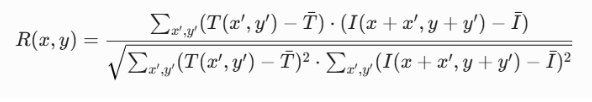
\includegraphics[width=0.7\textwidth]{figuras/coefcorr.png}
    \caption{Coeficiente de correlación normalizado con media cero.}
    \label{fig:coefcorr}
\end{figure}

Donde \emph{T} (\emph{Template}) es la matriz de la imagen de referencia tomada en la calibración,  e \emph{I} (\emph{Image}) es la matriz de la imagen del fotograma actual.

Como se puede observar en el numerador de la ecuación, a cada píxel se le resta el valor promedio matemático de su respectiva matriz (motivo por el cual recibe el nombre de \emph{media cero}). Esto es clave para el algoritmo de detección, ya que no evalúa la intensidad lumínica absoluta de un píxel, sino qué tan diferente es respecto a su entorno más cercano. Así, por ejemplo, si el rostro del usuario se ilumina súbitamente por una fuente externa, todos los píxeles de la imagen aumentarán su valor, pero la dispersión relativa entre ellos permanecerá constante. Esto le proporciona al sistema una total inmunidad frente a las variaciones incontrolables de la iluminación ambiental. 
Como se mencionó anteriormente, la imagen de referencia (\emph{Template}) tiene una resolución de 96x96 píxeles, mientras que el fotograma a analizar posee una resolución mayor, de 128x128 píxeles, a pesar de que en ambos casos la imagen del ojo es del mismo tamaño. El motivo de esta diferencia es lograr que la función de correlación no se aplique una sola vez, sino de forma iterativa, permitiendo que el molde realice un barrido completo sobre la imagen en vivo. Esto significa que el algoritmo comienza superponiendo las coordenadas de origen (\emph{X}=0, \emph{Y}=0) de ambas matrices y calculando la fórmula estadística, luego desplaza el molde un píxel hacia la derecha (\emph{X}=1, \emph{Y}=0), vuelve a aplicar la ecuación y repite este ciclo hasta cubrir toda el área del fotograma. Al finalizar este escaneo, se obtiene una nueva matriz bidimensional que contiene todos los coeficientes resultantes de estas sucesivas aplicaciones.

\emph{(Imagen ilustrativa del proceso de barrido)}

Este minucioso proceso de análisis se justifica por los inevitables errores de posicionamiento relativos entre el ojo y la cámara. Al utilizar una fórmula matemática tan estricta, si se evaluara una única posición estática, cualquier mínima perturbación del dispositivo (incluso de un milímetro), desalinearía las matrices y provocaría el fracaso inmediato del cálculo. Por lo tanto, realizar un barrido completo otorga un margen geométrico para compensar cualquier desplazamiento involuntario. Con esta técnica se logra una ventaja ergonómica fundamental para el proyecto: la inmunidad del sistema ante los micro-movimientos físicos de la cabeza del usuario.
De esta matriz resultante, con todos los valores de correlación, se extrae el coeficiente más alto (correspondiente al ciclo de comparación en el que la plantilla se alineó con mayor precisión sobre el fotograma capturado). Este proceso se repite con los cinco moldes restantes y, de esos seis valores máximos, se determina cuál fue el mayor, identificando así a qué acción corresponde la mirada actual.

\emph{(Imagen del log indicando el mayor parecido)}

Una vez identificada la acción de mayor probabilidad, el sistema aplica la siguiente lógica de control:

\begin{itemize}

\item Mirada hacia alguna opción (esquinas): La interfaz resalta visualmente esa opción y la guarda temporalmente en memoria como la última acción válida.

\item Mirada hacia el centro (zona neutra): El sistema mantiene iluminada la última opción válida seleccionada, permitiendo al usuario descansar la vista sin perder su progreso.

\item Parpadeo (Ojo cerrado): El algoritmo actúa como un disparador de confirmación, ejecutando la decisión final si existía una opción previamente seleccionada.

\end{itemize}

Si bien este método de detección resultó mucho más robusto y funcional que todos los anteriores, en la práctica presenta algunos errores. Por un lado, aunque el algoritmo estadístico es inmune a las variaciones lineales de luz ambiental, las sombras proyectadas por la inclinación de una fuente de luz externa entorpecen el procesamiento. Esto justificó la decisión de reutilizar el diodo LED infrarrojo (IR) en el diseño, garantizando una iluminación frontal uniforme y la consecuente ausencia de estas sombras. 
El otro inconveniente detectado fue la susceptibilidad a los falsos positivos. En ocasiones, el algoritmo resultaba demasiado permisivo y confundía las orientaciones del ojo. Para mitigar este efecto, se introdujo por código un \emph{umbral de similitud}. Esto implica que toda coincidencia probabilística inferior a este valor será automáticamente ignorada por el sistema. Por defecto, este umbral se estableció empíricamente en un 80\% (aunque el usuario puede ajustarlo en todo momento desde la propia interfaz web), solucionando el problema con gran eficacia. 

\emph{(Imagen del slider)}

Teniendo en consideración todo lo estudiado hasta el momento y habiendo superado múltiples ensayos empíricos, se concluye que este método de seguimiento basado en la similaridad de patrones es el más efectivo, estable y eficiente. Por lo tanto, esta es la solución implementada en el dispositivo final.

\section{Intercomunicación de hardware}

En esta sección se explora la manera en la que se comunican todos los dispositivos que actúan en el sistema final. Se hablará de los datos que se transmiten a través de dichos canales de comunicación y la forma en la que se transmiten.

\subsection{Clientes y servidores}

Como se aclaró en una sección previa, la arquitectura principal utilizada en este proyecto se denomina \emph{Cliente-Servidor}, donde los clientes realizan pedidos a través de los enlaces de comunicación (en este caso particular, comunicación Wi-Fi) y los servidores responden con datos.
Quien adopta el rol de servidor central es el segundo \emph{ESP32-S3}, que no realiza la tarea de captura de fotogramas. Sus funciones principales son:

\begin{itemize}

\item \keyword{Gestión de base de datos}: Alojar y administrar la información en una memoria microSD, accediendo a ella cada vez que un cliente solicita datos de usuarios, métricas o cuestionarios.

\item \keyword{Alojamiento web (Web Server)}: Contener los archivos estáticos de la aplicación web en su memoria mediante un sistema de archivos interno (como \emph{SPIFFS} o \emph{LittleFS}), para servirlos a los navegadores de los dispositivos que se conecten.

\item \keyword{Enrutamiento de video}: Actuar como puente o punto de interconexión para permitir la transmisión continua de fotogramas desde el módulo capturador (\emph{ESP32-CAM}) hacia el navegador del usuario.

\item \keyword{Lógica de negocio (Backend)}: Administrar permisos, validar sesiones, procesar peticiones HTTP, manejar la lectura/escritura en la base de datos y coordinar toda la lógica interna del sistema.

\end{itemize}

Por otro lado, los clientes son aquellos nodos de la red que carecen de las funciones de ruteo y almacenamiento central, limitándose a solicitar recursos al servidor para complementar el sistema. En este contexto existen dos tipos de clientes bien diferenciados.

Uno de ellos es el módulo \emph{ESP32-CAM}, el cual actúa como cliente de transmisión. Su función es solicitar un enlace en la red para enviar el flujo constante de fotogramas capturados.
Los demás clientes son los dispositivos de usuario finales (el celular del alumno, la computadora del profesor o la tablet de un tutor). Su función de hardware es simplemente proveer un navegador capaz de descargar y ejecutar la aplicación web (\emph{frontend}), donde se renderiza la interfaz visual. Para lograr esto y mantener el sistema operativo, estos dispositivos solicitan datos continuamente al servidor tales como el video en tiempo real, el estado de las sesiones, los cuestionarios activos o cualquier otra variable alojada en la base de datos necesaria para la ejecución del programa.

\emph{(Diagrama más específico del sistema)}


\subsection{Servidor Wi-Fi local (Naty)}

\subsection{Transmisión de datos (Naty)}

\section{Base de datos (Naty)}

\section{Aplicación web}

En esta sección se describen todas las funcionalidades de la aplicación web (\emph{frontend}) y el gestor encargado de asegurar su correcto funcionamiento (\emph{backend})

\subsection{Frontend}

El \emph{frontend} es la parte del código que se muestra ante el usuario. Su función es ser el intermediario entre el \emph{backend}, quien gestiona los datos y los permisos, y el usuario.
En este trabajo se optó por desarrollarlo en \emph{React}, una librería de \emph{JavaScript} de código abierto, creada y mantenida por \emph{META}, diseñada específicamente para construir interfaces de usuario (UI) dinámicas e interactivas para aplicaciones web. Es una herramienta muy versátil, ya que se puede utilizar en el entorno de \emph{Visual Studio Code}, y trabaja con arquitectura basada en componentes (CBA), lo cual vuelve al código más modular, ordenado y sencillo de depurar.
La estructura del programa se divide por páginas o pantallas. Cada pantalla cumple un conjunto limitado de funciones que conforman un subsistema común. Para funcionar requieren de dos archivos: un archivo \emph{.jsx} que declara y enlaza cada entidad con la función que deben cumplir (botones, campos de texto, títulos, entre otros) y un archivo \emph{.css} que describe el aspecto de cada una de estas entidades (el color de los botones, el tamaño del texto que contengan, la extensión de los campos de texto y otros).
Las pantallas se podrían dividir en tres categorías: 

\keyword{Pantallas de acceso universal}

Son aquellas interfaces a las que cualquier usuario puede acceder independientemente de su rol, permisos o jerarquía. En esta categoría se agrupan cuatro vistas principales: \emph{Home}, \emph{Login}, \emph{Invitado} y \emph{Alumno}. 
La pantalla \emph{Home} es la interfaz de bienvenida que el usuario visualiza instantáneamente al ingresar a la dirección IP del servidor local. Cuenta con un diseño minimalista que incluye un texto de presentación y dos botones de navegación para indicar qué tipo de usuario está ingresando. Si se presiona el botón destinado al estudiante, el sistema redirige a la pantalla \emph{Alumno}; caso contrario, el botón de usuario externo deriva el flujo hacia la pantalla \emph{Login}.

(Imagen Home)

La pantalla \emph{Login}, como su nombre indica, es aquella que los usuarios que no son alumnos utilizan para identificarse antes de comenzar su sesión con el dispositivo. Los usuarios con jerarquía (profesores y tutores) deben ingresar sus credenciales para acceder al núcleo del sistema. Esta vista incorpora un botón para registrar un usuario nuevo, el cual despliega un formulario que solicita datos personales (nombre, apellido, contacto), el rol deseado, la materia (exclusivo para el rol de profesor) y una palabra clave de administrador. Esta clave maestra es un requisito de seguridad indispensable para autorizar la creación de perfiles aptos para utilizar el dispositivo con fines académicos. 

(Imagen Login y otra con registro)

Otro botón importante es el de \emph{Recuperar contraseña}, que permite a cualquier usuario restablecer su contraseña en caso de haberla olvidado. Naturalmente, esta acción requiere de la palabra clave maestra. 

(Imagen de recuperar contraseña)

Finalmente, la interfaz de inicio de sesión ofrece un botón para ingresar directamente como invitado. Esta vía está pensada para aquellas personas del entorno del estudiante (amigos o familiares) que deseen establecer una comunicación informal sin necesidad de poseer un perfil registrado en la base de datos. Al seleccionar esta última opción, el usuario es redirigido a la pantalla \emph{Invitado}. Esta vista presenta un formulario simplificado de opción múltiple diseñado para estructurar preguntas rápidas.  Posee un campo para la pregunta, cuatro para las posibles respuestas, botones para eliminar o agregar opciones (hasta un máximo de cuatro) y un botón para enviar la pregunta al estudiante.

(Imagen de pantalla invitado)

Por último, se encuentra la pantalla \emph{Alumno}. Al tratarse del usuario principal y prioritario del sistema, su ingreso no requiere autenticación. Sus funciones exclusivas son calibrar la cámara y responder las evaluaciones que lleguen desde otros dispositivos. Al ingresar a esta vista, el usuario observa un panel indicador del estado del sistema y dos botones de acción principal (calibración y examen). Dichos botones permanecen bloqueados por seguridad hasta que el sistema esté en condiciones de operar. Para lograr esto, el frontend le solicita al servidor la descarga del archivo \emph{opencv.js}. Esta librería matemática actuará como el motor de la detección visual, pero adaptada exclusivamente para el método de similaridad de patrones (dejando atrás el enfoque previo de los círculos de Hough). 

(Imágenes de panel alumno bloqueado y desbloqueado)

Una vez que el indicador confirma que la librería \emph{OpenCV} fue leída desde la tarjeta microSD, transferida y compilada correctamente por el navegador, los botones de acción se habilitan. El primero de ellos dirige a la interfaz de calibración, la cual está compuesta por seis cuadros de previsualización vacíos, un recuadro de mayor tamaño donde se proyecta el flujo de video en vivo, y los comandos para iniciar o abortar el proceso. Si el sistema detecta una calibración almacenada previamente, advierte al usuario para evitar posibles redundancias.

(Imagen pantalla de calibración)

Al pulsar el botón de inicio, comienza una secuencia guiada para capturar los fotogramas de referencia: un indicador visual le señala al usuario hacia qué cuadrante debe dirigir la mirada y, tras una cuenta regresiva de tres segundos, el algoritmo captura la imagen. Este procedimiento se repite para todas las direcciones y para el parpadeo final. Una vez concluida la secuencia, los patrones capturados se exhiben en los cuadros de previsualización, otorgando la opción de guardar dicha calibración o reiniciar el proceso.

(Imagen de uno de los pasos de la secuencia)

El segundo botón del panel principal(\emph{Iniciar cuestionario}) redirige a la interfaz operativa de evaluación. Esta pantalla presenta el flujo de video en la esquina superior derecha junto a un control deslizante (\emph{slider}) que permite ajustar dinámicamente el umbral de sensibilidad del algoritmo. En este estado, el cliente aguarda pasivamente hasta que un invitado envíe una consulta o un profesor inicie formalmente un cuestionario. Al recibir los datos, la interfaz se actualiza automáticamente mostrando el enunciado y cuatro cuadrantes coloreados con sus respectivas opciones. Para responder, el alumno debe sostener la mirada hacia el cuadrante deseado (la interfaz lo resaltará visualmente) y ejecutar un parpadeo intencional para confirmar el registro en la base de datos. Adicionalmente, el usuario puede retornar la mirada a la zona neutra (centro) para descansar la vista o revisar su elección sin alterar la selección previa. En paralelo a este proceso, el sistema cliente emite señales periódicas al servidor (heartbeats) para mantener activa la sesión de forma ininterrumpida, permitiendo que el microcontrolador contabilice con precisión el tiempo total empleado en la resolución. 

(Imagenes de todas las posibles pantallas de cuestionario)

Si la pregunta provino del modo \emph{Invitado}, la sesión concluye inmediatamente mostrando la respuesta enviada. Si se trata de un examen oficial, el sistema muestra todas las preguntas en orden hasta alcanzar la pantalla final, donde se expone el puntaje obtenido, el tiempo transcurrido y la condición de aprobación. Cabe destacar que el profesor posee control total sobre el flujo del examen, pudiendo pausarlo, reanudarlo o finalizarlo remotamente en cualquier momento, lo cual fuerza la actualización inmediata de la pantalla del alumno hacia los estados correspondientes.

\keyword{Pantallas de acceso restringido}

Son aquellas interfaces a las que solo pueden acceder los usuarios registrados mediante el ingreso de sus credenciales (nombre de usuario y contraseña). A todas estas vistas se accede de forma exclusiva superando la validación de la pantalla de login. Si el servidor central (\emph{ESP32}) detecta que un dispositivo intenta conectarse a estas rutas sin poseer un token de sesión activo y válido, el sistema emite una alerta de seguridad y redirige automáticamente al usuario de regreso a la pantalla de inicio de sesión. También posee un límite de tiempo que cierra la sesión automáticamente tras varios minutos de inactividad. En esta categoría se agrupan las pantallas: \emph{Panel}, \emph{Perfil}, \emph{Contactos} y \emph{Cuestionarios}. 

La pantalla \emph{Panel} es la interfaz principal que el usuario visualiza inmediatamente tras autenticarse con éxito. Presenta un encabezado con un texto de bienvenida que incluye el nombre y apellido del usuario activo, junto a un botón rojo destinado a cerrar la sesión en cualquier momento. A continuación, se despliegan tres grandes botones de navegación cuyo contenido es dinámico y depende de la jerarquía de la cuenta:

Si el usuario posee el rol de profesor, visualizará las opciones: \emph{Ver cuestionarios}, \emph{Ver datos tutor} y \emph{Editar perfil}.
En cambio, si el usuario es un tutor, el botón intermedio se adapta a su necesidad y es reemplazado por la opción \emph{Ver profesores}.

(Imagenes de pantalla panel para ambos usuarios)

El botón \emph{Editar perfil}, común a ambos roles, redirige a la pantalla \emph{Perfil}. Esta vista tiene como objetivo ofrecer al usuario la posibilidad de modificar su información personal en todo momento. Al igual que en el panel principal, conserva el encabezado de bienvenida y el botón de cierre de sesión. Debajo de estos elementos, presenta un formulario estructurado con campos de texto para actualizar los siguientes datos: nombre de usuario, nombre, apellido, contacto y, exclusivamente para profesores, la materia. Los cambios realizados en este segmento se envían a la base de datos al pulsar el botón \emph{Guardar datos}.

(Imagen del primer formulario)

Seguidamente, la interfaz dispone de una sección independiente dedicada a la actualización de credenciales. Para cambiar la contraseña, el sistema solicita ingresar la clave actual seguida de la nueva, omitiendo la necesidad de utilizar la palabra clave maestra, dado que la identidad del usuario ya se encuentra validada por su sesión activa.
En la parte inferior, la interfaz provee un botón rojo diseñado para eliminar definitivamente la cuenta del usuario activo. Como medida de seguridad, al accionar este botón el navegador despliega un cuadro de diálogo de confirmación antes de ejecutar el borrado en la base de datos. Finalmente, existe un botón de navegación para regresar al panel anterior, el cual cuenta con una validación interna que advierte al usuario si intenta abandonar la vista existiendo modificaciones sin guardar.

(Imagen del resto)

Retornando al menú principal, el botón central dirige a la pantalla \emph{Contactos}, cuya interfaz y funcionalidad son dinámicas y se adaptan al rol del usuario activo en la sesión.
Si el usuario posee el rol de profesor y accede mediante la opción \emph{Ver datos tutor}, visualizará una pantalla encabezada por el título \emph{Datos del Tutor}. Debajo, se despliega una tarjeta informativa que contiene los datos básicos del tutor asociado al dispositivo del alumno: nombre, apellido y contacto. Si la base de datos no registra ningún tutor, la interfaz oculta la tarjeta y advierte al usuario mediante un mensaje de texto indicando la ausencia de este perfil. Cabe mencionar que cada tutor debe ser único por cada dispositivo, por lo que se muestra siempre una única tarjeta en caso de haberlo.

(Imagen de ver tutores)

Por el contrario, si el usuario autenticado es un tutor e ingresa mediante el botón \emph{Ver profesores}, el encabezado cambia a \emph{Profesores} y la vista presenta una lista dinámica. Esta lista renderiza, en formato de tarjetas individuales, la información de todos los docentes registrados en el dispositivo, detallando para cada uno: Materia, nombre, apellido y contacto. Asimismo, cada tarjeta incorpora un botón de acción destructiva que permite al tutor eliminar manualmente a cualquier profesor del sistema. Al accionar este comando, la interfaz exige una confirmación explícita antes de ejecutar el borrado definitivo en la base de datos (acción que, por diseño del servidor, elimina en cascada los cuestionarios asociados a dicho docente). Al igual que en la vista anterior, si no existen profesores registrados, se notifica la situación con un breve texto en pantalla.

(Imagen de ver profesores)

Finalmente, cabe destacar que, a diferencia del panel principal, esta interfaz prescinde del encabezado de bienvenida y del botón de cierre de sesión, priorizando una visualización limpia que ofrece únicamente un botón inferior denominado \emph{Volver} para retornar de forma segura al menú anterior.
La pantalla \emph{Cuestionarios}, accesible a través del panel principal, constituye el núcleo de la gestión académica del dispositivo, presentando múltiples variaciones funcionales dependiendo de la jerarquía del usuario.
Para el profesor, esta pantalla actúa como el motor integral de las evaluaciones: permite crearlas, modificarlas, controlar su ejecución en tiempo real y eliminarlas. La vista inicial consiste en un listado dinámico de todos los cuestionarios asociados a su materia. Cada elemento de la lista expone datos clave: título, cantidad de preguntas, puntaje obtenido y su condición final (aprobado o desaprobado). El control de cada módulo se gestiona a través de cuatro botones, los cuales se habilitan o deshabilitan respondiendo a la máquina de estados del servidor:

\begin{itemize}

\item Estado \keyword{PENDIENTE} (Previo a la ejecución): Se habilitan los botones superiores de acción destructiva/modificadora (\emph{Editar} y \emph{Eliminar}). En el bloque inferior, se habilita el botón \emph{INICIAR} (cuyo accionamiento transiciona el examen al estado \emph{En Progreso}) y se mantiene bloqueado el botón \emph{FINALIZAR}.

\item Estado \keyword{EN PROGRESO} (Alumno respondiendo: Para garantizar la integridad de los datos, el sistema bloquea inmediatamente los botones de edición y eliminación. El botón de inicio asume la función de \emph{PAUSAR}, y se habilita el botón de \emph{FINALIZAR} como mecanismo de aborto seguro en caso de contingencias.

\item Estado \keyword{PAUSADO}: Los controles superiores de edición permanecen bloqueados y el botón de finalización sigue activo. El botón de estado muta a \emph{REANUDAR}, permitiendo al alumno continuar el examen desde la última pregunta contestada.

\item Estado \keyword{FINALIZADO}: Los botones de edición y finalización se desactivan. Se rehabilita la capacidad de eliminar el registro, y el botón de estado principal se transforma en “REVISAR”, redirigiendo al profesor a las analíticas del examen.

\end{itemize}

(Imagen de pantalla cuestionarios de profesor)

Por encima de este listado, un botón etiquetado como \emph{Nuevo +} da acceso a la interfaz de creación y edición. Esta vista presenta una plantilla estructurada encabezada por el título del cuestionario (editable de forma interactiva). A continuación, se despliegan los bloques de las preguntas, los cuales permiten ingresar la incógnita y configurar dinámicamente entre dos y cuatro opciones posibles.

A nivel de configuración, el docente puede seleccionar la respuesta correcta mediante un botón de selección, establecer el puntaje a sumar por acierto y definir el puntaje a restar por error. Para optimizar la carga de datos, la interfaz incluye herramientas de diseño que permiten replicar un mismo esquema de puntajes a todo el examen (\emph{Aplicar a todas}), reordenar la posición de las preguntas en la lista mediante flechas direccionales, o eliminar preguntas enteras. En el margen inferior, se encuentra un campo numérico para establecer el umbral de aprobación y los tres comandos de cierre: \emph{Añadir Pregunta}, \emph{Guardar Cuestionario} (que empaqueta los datos y los envía al ESP32) y \emph{Volver sin guardar}.

(Imagenes de la pantalla del editor)

Retornando al flujo principal, cuando un cuestionario finalizado es sometido a revisión (mediante el botón \emph{REVISAR}), el sistema despliega una vista analítica. Esta pantalla detalla el tiempo total empleado, el puntaje final, la condición de aprobación, un desglose pregunta por pregunta indicando la opción elegida por el alumno, la opción correcta (si hubo equivocación) y el impacto numérico de dicha respuesta en el puntaje total.

(Imagenes de la vista de revision)

Finalmente, si el usuario que accede a esta sección posee el rol de tutor, la interfaz restringe severamente sus privilegios. El listado mostrará los cuestionarios históricos creados por la totalidad de los profesores, indicando adicionalmente a qué materia pertenece cada uno. Todos los controles de edición, eliminación y alteración de estados se suprimen gráficamente. El tutor únicamente cuenta con el botón de \emph{REVISAR} para consultar las analíticas, el cual permanecerá bloqueado hasta que el sistema registre que el cuestionario ha alcanzado el estado \emph{FINALIZADO}.

(Imagen de la pantalla cuestionarios del tutor y otra de la pantalla de revisión)


\keyword{Núcleos de la aplicación}

A diferencia de las interfaces visuales descritas anteriormente, esta categoría abarca los archivos y scripts estructurales que operan en segundo plano. No poseen una representación gráfica directa para el usuario, pero constituyen el motor lógico que sostiene la arquitectura de \emph{Aplicación de Página Única} (SPA, por sus siglas en inglés) y gestionan la comunicación con el servidor central.

(Imagen de los archivos nucleo en el visual studio)

El punto de entrada (\keyword{index.html} y \keyword{main.jsx}):  En el paradigma SPA, el servidor \emph{ESP32} aloja y transmite un único documento \emph{HTML} (\emph{index.html}) que actúa como un lienzo en blanco. El archivo \emph{main.jsx} es el script principal de inicialización. Su única y vital función es inyectar la librería \emph{React} dentro de ese documento HTML vacío, montar el \emph{Virtual DOM} (Modelo de Objetos del Documento Virtual) y comenzar a renderizar los componentes de la interfaz a la velocidad del procesador del cliente, evitando que la página web deba recargarse al navegar. Como detalle adicional, el archivo \emph{index.html} también se encarga de descargar el script de \emph{OpenCV} (\emph{opencv.js}, almacenado en la tarjeta microSD) para que esté disponible globalmente en la aplicación. 

El gestor de rutas (\keyword{App.jsx}): Este componente actúa como el controlador de tráfico del sistema. Su función es evaluar continuamente la URL actual del navegador y decidir qué pantalla visual debe renderizarse en cada momento. Además, gestiona la lógica de protección de rutas: antes de permitir que un componente de acceso restringido se monte en pantalla (como el panel o los cuestionarios), \emph{App.jsx} verifica la memoria de sesión (\emph{sessionStorage}) en busca de un token de autorización válido. Si las credenciales no existen o caducaron, bloquea la navegación y redirige el flujo forzosamente hacia la pantalla de \emph{Login}. Además de controlar la navegación, este archivo implementa un monitor de sesión que vigila la inactividad del usuario (10 minutos) y realiza peticiones periódicas (\emph{/api/auth/heartbeat} cada 5 segundos) para asegurar que el token sigue siendo válido en el servidor. Si la validación falla, ejecuta la función \emph{handleLogout}, la cual limpia las credenciales y redirige a la pantalla de inicio de sesión para proteger las herramientas administrativas. 

La capa de servicios (\keyword{services/api.js}): Para mantener una arquitectura de software escalable y ordenada, el sistema aísla todas las comunicaciones de red en un módulo de servicios independiente. Este script centraliza todas las peticiones asíncronas (HTTP y REST) dirigidas al backend alojado en el \emph{ESP32}. Su existencia permite que los componentes gráficos soliciten datos (como el estado de un examen o la lista de profesores) invocando funciones simples, mientras este archivo se encarga de la complejidad de estructurar las cabeceras de red, adjuntar los tokens de seguridad y parsear las respuestas JSON provenientes del microcontrolador.

Compilación y despliegue (\keyword{dist/}): Cabe destacar que el código fuente desarrollado en React no puede ser interpretado nativamente por los navegadores ni almacenado de forma eficiente en un microcontrolador. Por este motivo, el proyecto utiliza una herramienta de construcción (en este caso, \emph{Vite}) que compila, minimiza y empaqueta todo el código fuente en un conjunto de archivos estáticos altamente optimizados (ubicados en el directorio \emph{dist/}). Son exclusivamente estos archivos livianos los que finalmente se transfieren a la memoria microSD del \emph{ESP32} principal para ser servidos a los usuarios.


\subsection{Backend (Naty)}

\section{Interfaz de usuario táctil}

Con el fin de aumentar y mejorar la accesibilidad al momento de utilizar el dispositivo, se optó por incorporar una interfaz visual directamente en el microcontrolador servidor. En el mercado existen diversas variantes de módulos \emph{ESP32} que difieren según sus periféricos integrados. Uno de ellos es el modelo \emph{ESP32-2432S028}, conocido coloquialmente como \emph{ESP32-CYD} (\emph{Cheap Yellow Display}). Este hardware incorpora el mismo procesador utilizado a lo largo de este proyecto, con el agregado particular de una pantalla LED táctil integrada.

(Imagen de CYD)

Este componente permite renderizar elementos interactivos como textos, imágenes, botones y teclados virtuales, mejorando significativamente la experiencia de usuario de forma autónoma (sin depender de un dispositivo externo). Para gestionar y dibujar esta interfaz gráfica, el sistema emplea dos librerías fundamentales:

\begin{itemize}

\item \keyword{TFT\_eSPI}: Otorga los controladores (drivers) de bajo nivel necesarios para la comunicación por hardware con el display.

\item \keyword{LVGL}: Es una librería gráfica de alto nivel que permite renderizar y gestionar la lógica de los elementos visuales y las interacciones táctiles del usuario.

\end{itemize}

A nivel arquitectónico, la interfaz se divide en dos grandes bloques lógicos: un contenedor deslizante (\emph{TileView}) que agrupa tres vistas de uso continuo, y una cuarta vista aislada destinada a la configuración inicial del sistema. Toda la información necesaria la consigue mediante comandos sencillos que comunican el backend con el frontend.

\keyword{Vista 1 - Bienvenida}

Es la primera interfaz que visualiza el usuario al encender el dispositivo ya configurado. Su diseño es minimalista y consta de un texto de bienvenida acompañado de un código QR. Al escanear este código con cualquier teléfono móvil, el usuario es redirigido automáticamente a la URL local del servidor (\emph{levi.local}), simplificando el acceso y evitando la introducción manual de direcciones IP. 

(Imagen vista 1)


\keyword{Vista 2 - Estado del sistema}

Al deslizar la pantalla hacia la derecha, se accede a un panel de monitoreo. Su función es exponer en tiempo real los datos críticos sobre el funcionamiento de la red local y los nodos conectados. La información expuesta incluye:

\begin{itemize}

\item Nombre del alumno propietario del dispositivo.
\item Nombre del usuario administrativo (profesor o tutor) con sesión activa.
\item Estado del módulo de captura visual (indicando si la cámara está \emph{Transmitiendo} o \emph{Desconectada}).
\item Cantidad total de clientes conectados al servidor.

\end{itemize}

En condiciones normales de uso deberían haber tres dispositivos conectados: el alumno, el profesor y la cámara.

(Imagen vista 2, varias posibilidades)

\keyword{Vista 3 - Examen}

Es la última pantalla del flujo continuo. Su propósito es brindar un seguimiento de las evaluaciones activas, permitiendo al docente (u observador externo) conocer el progreso del alumno directamente desde la carcasa del dispositivo. Cuando no hay cuestionario activo, esta pantalla está en modo de espera, con un texto azul centrado que indica \emph{'Esperando cuestionario'}

Cuando hay un cuestionario activo, la pantalla cambia mostrando su título y el progreso actual del alumno.

\keyword{Vista 4 - Inicialización}

A diferencia de las anteriores, esta vista se ejecuta de manera exclusiva durante el primer arranque del equipo (o tras un formateo de fábrica). Su objetivo es configurar las credenciales permanentes del sistema operativo. Mediante el uso de un teclado táctil virtual desplegable, el administrador debe ingresar tres parámetros vitales: el nombre del alumno, la palabra clave maestra para profesores y la palabra clave maestra para tutores.
Estas credenciales actúan como la raíz de seguridad del dispositivo. Una vez completados los campos, el usuario debe oprimir el botón de guardado, el cual almacena las variables de forma persistente en la memoria no volátil (NVS) del microcontrolador y fuerza un reinicio automático del sistema, cargando finalmente la vista de bienvenida convencional.

(Vista pantalla de booteo)


\section{Alimentación}

Entre las premisas de este trabajo se estipuló que el dispositivo final debe ser inalámbrico y autosuficiente en términos de consumo energético al momento de utilizarlo. Siguiendo estos lineamientos, se opta por no alimentarlo utilizando cables y entradas USB-C o MicroUSB que se incluyen en los modelos comerciales de los microcontroladores utilizados, sino que se diseñará su propio sistema de alimentación utilizando fuentes de energía independientes de cualquier dispositivo externo al momento de uso. La solución general planteada para este problema recae en el uso de las baterías de litio, una de las fuentes de energía inalámbrica más comunes en los dispositivos electrónicos de bajo consumo. A pesar de su precio relativamente elevado a comparación de las pilas comunes, tienen la particularidad de que son recargables, evitando así que el usuario tenga que comprar repuestos en el momento en que se agote la energía. 

La alimentación a través de estas pilas permitirá un uso prolongado del dispositivo antes de necesitar una recarga y al mismo tiempo evita la necesidad de comprar pilas comunes para cada período de uso. La energía suministrada será moldeada por otros componentes electrónicos para obtener la salida continua y estable que requieren estos microcontroladores para funcionar correctamente. Cada placa (emisora de la gorra y CYD receptora) tendrá su propio circuito de alimentación independiente de la otra, para así evitar enlazar ambas partes del proyecto mediante un cable y poder mover a la CYD con la interfaz libremente. En esencia, ambos circuitos serán exactamente iguales, pues se trata con dos microcontroladores que, para su uso en este contexto, requieren de la misma señal de alimentación.

Teniendo seleccionada la fuente de energía, se presentan otros dos problemas. Se requiere una forma para recargar las pilas de manera sencilla, y además un método para estabilizar la señal de alimentación. Esto último se debe a que los \emph{ESP32} requieren una alimentación de 3,3 V o, en su defecto, de 5 V lo más estables posible, ya que una mala alimentación puede provocar mal funcionamiento, reinicios inesperados o destrucción del hardware. 

\subsection{Soluciones propuestas}

\keyword{1- Alimentación directa + Regulador lineal de tensión + Cargador de pilas externo}

Consiste en alimentar el microcontrolador directamente desde la pila de litio a través de un portapilas. A esto se le suma un regulador de tensión lineal de baja caída (LDO), como el \emph{AMS1777}, para ajustar la tensión a 3,3 V estables. Para recargar las pilas se emplearía un cargador comercial externo, que requiere extraer físicamente la pila del dispositivo para colocarla en la ranura y conectarla a la red.

(Imagen del LDO)

Ventajas de esta solución:

\begin{itemize}

\item Mantenimiento práctico: Los cargadores comerciales son componentes estándar y fáciles de conseguir en el mercado.

\item Optimización de espacio: Al requerir únicamente un portapilas, el regulador lineal y un par de capacitores de filtrado, se reduce considerablemente el espacio ocupado en una PCB.


\end{itemize}


Desventajas de esta solución:

\begin{itemize}

\item Ergonomía y desgaste mecánico: Resulta impráctico para el usuario el tener que retirar la pila del dispositivo cada vez que se quiera recargar, además de que esto puede provocar desgaste mecánico con el tiempo.

\item Descarga de la pila: Una pila de litio estándar (como la \emph{18650}) de 3,7 V no entrega este valor continuo de tensión a lo largo del tiempo, sino que disminuye progresivamente hasta llegar a un piso mínimo de unos 3,0 V. Este valor es menor a los 3,3 V que necesita el microcontrolador, lo que significa que el dispositivo dejaría de funcionar mucho antes de que la batería se quede sin energía para dar. Se requiere hardware adicional para aumentar el valor de tensión cuando sea necesario, y agregarlo invalida la ventaja de la optimización de espacio.

\item Dropout: La función del regulador es estabilizar la tensión en 3,3 V. Sin embargo, estos integrados operan con transistores MOSFET en zona activa (es decir, actuando como resistencias variables), lo que implica inevitablemente que habrá una caída de voltaje entre la entrada y la salida. Esta caída se llama \emph{voltaje de dropout}, lo que significa que para tener 3,3 V estables a la salida, necesitaremos una tensión continua mayor que ese valor en la entrada, lo que reduce aún más el tiempo en el que se puede usar el dispositivo antes de que la pila se quede sin energía.

\item Picos de corriente: El consumo de corriente de una \emph{ESP32} es dinámico. Hay ocasiones, como al encender el Wi-Fi, en las que el microcontrolador exige grandes transitorios o picos de corriente de hasta 500 mA. Por ley de ohm, al exigir más corriente al regulador, la caída de tensión de dropout por la resistencia del silicio se maximizará. Esto agrava el problema anteriormente mencionado, provocando caídas bruscas en la tensión de alimentación que disparan el detector de bajo voltaje (\emph{brownout detector}) del microcontrolador.

\end{itemize}


\keyword{2- Placa de alimentación (Módulo TP4056 + Módulo MT3608)}

El módulo \emph{TP4056} es un circuito integrado utilizado para recargar baterías como las que se usarán en este proyecto, mientras que el \emph{MT3608} es un módulo elevador de voltaje (boost) que entrega a la salida una señal muy estable del valor elegido por el diseñador. Si se interconectan ambos módulos se formaría un conjunto que cumpliría los requisitos de recarga y regulación, y se podría alimentar al \emph{ESP32} desde el pin de 5 voltios.

(Imagen de los modulos en cuestión)

Ventajas:

\begin{itemize}

\item Facilidad de mantenimiento: Al ser dos módulos separados, las fallas puntuales pueden repararse fácilmente utilizando un repuesto del módulo necesario sin alterar el sistema completo.

\item Carga térmica: Al ser dos módulos diferentes que se encargan de distintas tareas, la temperatura que alcance cada uno será independiente del otro y se distribuirá uniformemente a lo largo de la PCB.

\item Sin dropout ni picos de corriente: El módulo \emph{MT3608} es un regulador switching, que utiliza transistores MOSFET en zona de corte y saturación, por lo que no hay caídas apreciables de tensión entre la entrada y la salida. A su vez, los picos de corriente pueden ser abastecidos por el ajuste automático del ciclo de trabajo del switch.

\item Doble regulación de tensión: Al alimentar el \emph{ESP32} a través del pin de 5 V, se utiliza el regulador integrado en la placa para reducirlos a 3,3 V aún más estables.

\end{itemize}

Desventajas:

\begin{itemize}

\item Mantenimiento impráctico: A pesar de que las reparaciones son más sencillas y baratas, los módulos mencionados sólo pueden conseguirse en casas especializadas en electrónica, a diferencia del cargador estándar.

\item Menor optimización del espacio: Al tener dos módulos distintos, se requiere una PCB más espaciosa para contenerlos.

\item Pérdida de eficiencia: La ventaja de la doble regulación implica inevitablemente una pérdida de eficiencia. La energía sufre dos conversiones: de la pila a los 5 V y de los 5 V a los 3,3 V en el regulador interno del \emph{ESP32}, lo que aumenta la disipación térmica.

\end{itemize}

\keyword{3- Placa de alimentación con un regulador Buck-Boost}

Se podría pensar que para evitar esa pérdida de eficiencia con el \emph{MT3608} y alimentar al microcontrolador con 3,3 V se pudiera utilizar un regulador Buck-Boost (como el \emph{XL6009}) en lugar del elevador Boost para alimentarlo a 5 V. Pero la ventaja de la eficiencia contrasta con el aumento del costo y la complejidad del circuito integrado. Más adelante se realizará un análisis de mercado para comprobar este punto.

(Imagen del BuckBoost)

\keyword{4- Integrado \emph{Power Bank} todo en uno}
El integrado \emph{IP5306} cumple la misma función que la placa de alimentación utilizando un solo chip integrado que realiza internamente el proceso de carga y de regulación de tensión.

(Imagen del IP5306)

Ventajas:

\begin{itemize}

\item Optimización del espacio en PCB al ser un solo módulo.

\item Regulación conmutada: Al igual que los elevadores y reductores, funcionan con transistores en zona de corte y saturación, evitando el problema del dropout y los picos de corriente.

\item Carga y uso simultáneo.

\end{itemize}

Desventajas:

\begin{itemize}

\item Mantenimiento impráctico, por la dificultad agregada de conseguir los repuestos.

\item Pérdida de eficiencia por usar doble regulación.

\item Carga térmica: Al ser un solo chip el que hace la tarea de carga de batería y regulación de voltaje, todo el calor disipado se acumulará en un único punto del dispositivo, lo que influirá negativamente en el funcionamiento del mismo.

\item No es modular: Si se produjera una falla en cualquier parte del sistema, inevitablemente habría que comprar el repuesto completo del chip, lo cual es más costoso que comprar los repuestos separados de los módulos anteriormente vistos.

\item Ripple en la señal de salida: Al estar diseñados para cargar celulares conectándose a un PMIC interno, los chips \emph{IP5306} conmutan a mucha menor frecuencia (entre 300 y 500 kHz), que el módulo \emph{MT3608}, por ejemplo. Además, carece de filtros adecuados a la salida, lo que provoca que este rizado sea más difícil de eliminar. Este ripple es sumamente indeseable para alimentar un servidor Wi-Fi y una cámara que debe transmitir en vivo. 

\end{itemize}

Para solucionar el problema del ripple, se podría utilizar directamente un PMIC industrial, pero su elevado costo y la complejidad de soldadura de sus encapsulados lo vuelven inviable para este prototipo. 

\keyword{Análisis de mercado}

(Tabla con las comparaciones de precios)


\subsection{Descripción del sistema elegido}

El primer circuito integrado que utilizaremos es el chip \emph{TP4056}, cuyo datasheet lo describe como un cargador lineal de corriente constante/tensión constante completo para baterías Li-ion de una sola celda. Este chip toma energía de una fuente externa y la adapta para recargar la batería. La energía que proveen estas baterías de larga duración suele ser de 3,7 voltios. Por lo tanto, para adecuar y estabilizar este nivel de tensión se utiliza otro circuito integrado fundamental: el \emph{MT3608}; el cual, en términos sencillos, se trata de un circuito elevador boost que en la salida entrega una señal continua y estable según el ajuste que realice el diseñador. Esa salida irá directamente conectada a la entrada de 5 voltios de la placa \emph{ESP32}.

El funcionamiento en detalle de estos integrados y sus módulos comerciales serán descritos en las siguientes secciones.


\subsection{Recarga y protección}

Como se expuso con anterioridad, el chip \emph{TP4056} sirve para cargar una única celda de baterías de litio, y lo hace en un ciclo de dos fases.

En primera instancia carga la batería a corriente constante, es decir, le inyecta un valor fijo de corriente elegida por el diseñador para que la carga comience siendo rápida. Al mismo tiempo, el chip mide constantemente el voltaje de la pila, y cuando llega a los 4,2 V comienza la fase de carga con voltaje constante, y permite a la propia pila que absorba la corriente necesaria para no destruirse. Si toda la carga fuera a corriente constante, se le inyectaría a la pila más energía de la que puede soportar y acabaría destruyéndose. Por el contrario, si toda la carga fuese a voltaje constante, el proceso llevaría demasiado tiempo, lo cual es poco práctico para la experiencia de usuario. Es por eso que este integrado oscila automáticamente entre esos dos modos.

Por otra parte, el \emph{TP4056} está diseñado para detener la carga en la fase de voltaje constante, cuando la corriente absorbida por la pila sea inferior a una décima del valor programado por el usuario, lo cual evita sobrecargar la pila.

Para resumir, sus características más relevantes son:

\begin{itemize}

\item Corriente de carga programable hasta 1000 mA.
\item Operación dinámica entre corriente constante y voltaje constante.
\item Carga hasta un valor fijo de 4,2 V.
\item Fin de carga automático.
\item UVLO.
\item Umbral de carga lenta.
\item Arranque suave de corriente.

\end{itemize}

UVLO (\emph{Under Voltage Lockout} / Bloqueo por bajo voltaje): Es una funcionalidad del chip que permite que cuando se introduzca una alimentación mala o inestable, la carga se bloquee para evitar que el proceso dañe la pila o los circuitos.

Umbral de carga lenta: Para evitar sobrecargar una pila en mal estado (con voltaje inferior a 3,0), el \emph{TP4056} entra en modo \emph{carga lenta}, enviando solo el 10\% de la corriente programada hasta que supere el umbral. Luego de eso la carga procede con normalidad.

Arranque suave de corriente: Es una medida de protección a la fuente externa. Garantiza que al enchufar el circuito a la misma, la absorción de corriente no sea tan brusca, sino que aumente gradualmente con el tiempo para evitar daños.

Su diagrama de pines es el siguiente:

\begin{figure}[htbp]
    \centering
    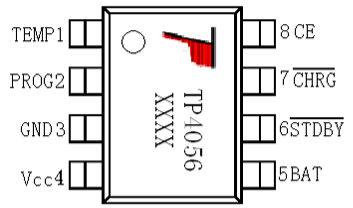
\includegraphics[width=0.5\textwidth]{figuras/tp4056pinout.png}
    \caption{Diagrama de pines del módulo \emph{TP4056}}
    \label{fig:tp4056pinout}
\end{figure}


\begin{enumerate}

\item TEMP: Entrada de sensor de temperatura. Sirve para monitorear la temperatura de la pila al momento de la carga mediante un termistor externo. Debido al uso que se le va a dar en este proyecto y a la presencia de otros circuitos de protección, se opta por prescindir de su uso.

\item PROG: Entrada de programación de corriente de carga. A este pin se le debe conectar una resistencia denotada como \emph{RPROG} para establecer el valor de la corriente de carga. El valor esta se calcula con la siguiente fórmula:

\begin{equation}
Rprog = 1200*Ibat
\end{equation}

Donde \emph{Ibat} es la corriente en miliamperios elegida por el diseñador, con un valor máximo de 1000 mA.

\item GND: Tensión de referencia.

\item VCC: Entrada de alimentación externa.

\item BAT: Salida que se conecta al terminal positivo de la pila. Le brinda la corriente necesaria y regula el voltaje a 4,2 V.

\item STDBY: Salida en alta impedancia que se vuelve nula cuando la carga está completa.

\item CHRG: Salida en alta impedancia que se vuelve nula mientras la pila se está cargando.

\item CE: Habilitación del chip. Conectándolo a un 0 lógico se bloquean todas las funcionalidades del chip (Modo \emph{shutdown}).

\end{enumerate}

En el siguiente gráfico se ilustran las fases de corriente constante y voltaje constante descritas anteriormente:

\begin{figure}[htbp]
    \centering
    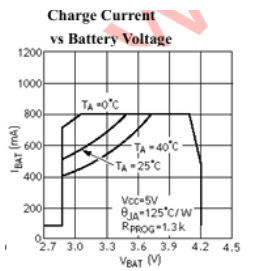
\includegraphics[width=0.5\textwidth]{figuras/tp4056grafico.png}
    \caption{Corriente vs voltaje de carga}
    \label{fig:tp4056grafico}
\end{figure}

Con un voltaje menor a 4,2 V, se programó en ese caso una corriente de 800 mA. El ciclo comienza con un aumento gradual de la corriente hasta llegar a ese valor programado. El voltaje mientras tanto va aumentando, y al llegar a los 4,2 V, la corriente disminuye con ese mismo valor hasta finalizar la carga.

Se explica a continuación un circuito de uso típico con este chip, correspondiente al módulo que se encuentra comercialmente en las casas de electrónica y se utiliza en este proyecto:

\begin{figure}[htbp]
    \centering
    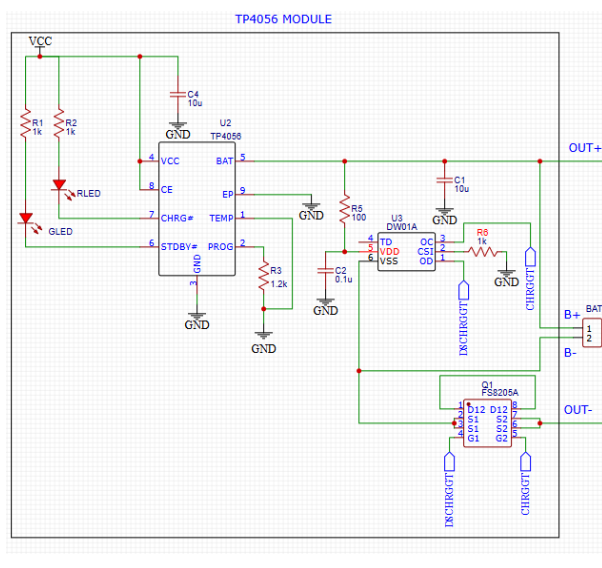
\includegraphics[width=0.7\textwidth]{figuras/tp4056placa.png}
    \caption{Circuito típico de aplicación del \emph{TP4056}}
    \label{fig:tp4056placa}
\end{figure}

Lo primero que se puede notar es un puente entre la entrada CE y VCC, esto es debido a que para este uso práctico no se requiere deshabilitar el chip manualmente. Se observa también un capacitor C4 utilizado para drenar el ruido de la entrada

En las salidas CHRG y STDBY están conectados los cátodos de dos diodos LED. Uno verde para STDBY y uno rojo para el CHRG. Estos son LEDs indicadores que informan al usuario en qué estado se encuentra la carga.

En el pin PROG se conecta una resistencia RPROG (o R3 en el diagrama) de 1.2 kΩ, que es el valor por defecto comercialmente, lo que implica una corriente de carga programada de 1 A, y una corriente de corte de 100 mA.

El pin de sensor de temperatura se conectará a GND ya que no se utiliza, al igual que el pin 9 (EP), que sirve para disipación.

El pin 5 (BAT), no va conectado únicamente a la pila, sino que además pasa por un capacitor de desacople (C1) y por otros dos integrados que vienen conjuntos en el módulo: El \emph{DW01A} y el \emph{FS8205A}. 

El \emph{DW01A} es básicamente un monitor del voltaje y corriente de la pila. Si nota que el voltaje de la pila es inferior o superior a lo esperado, o detecta algún cortocircuito, le informa al \emph{FS8205A} mediante los pines CHRGGT y DSCHRGGT, para que este último actúe desconectando físicamente la pila del circuito mediante la salida B-.

Cuando todo está en condiciones, la pila se conecta mediante los terminales B+ y B- al pin BAT y a GND respectivamente. Si el integrado \emph{FS8205A} actúa, se abre un MOSFET aislando el terminal B- de GND y por lo tanto abriendo el circuito de carga.

\subsection{Estabilización de voltaje}

El chip \emph{MT3608} es un circuito \emph{Convertidor Step-up de alta eficiencia}. O más coloquialmente conocido como \emph{Elevador de tensión}. Su función es complementarse con un circuito externo típicamente conocido como \emph{Elevador boost} para tomar un determinado valor de voltaje a la entrada y obtener a su salida un valor más grande y más estable, listo para alimentar el microcontrolador.

Para entender su funcionalidad, debemos describir la función de un circuito elevador Boost, que se muestra a continuación:

\begin{figure}[htbp]
    \centering
    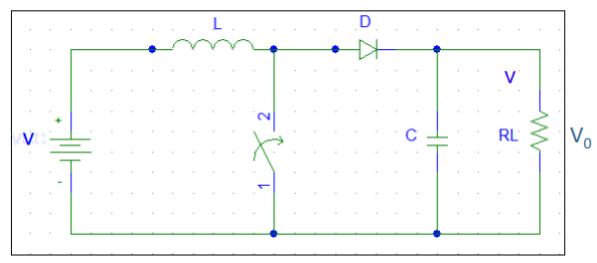
\includegraphics[width=0.7\textwidth]{figuras/boost.png}
    \caption{Circuito elevador Boost}
    \label{fig:boost}
\end{figure}

Este circuito es el típico que se utiliza para las fuentes de tensión tipo \emph{switching}. En este caso particular, la tensión continua de la entrada es la salida de la pila de Litio, que oscila entre 3,0 y 3,7 V. Esta señal pasa por un conjunto de una bobina, un diodo, un capacitor, y un switch que se abre y cierra intermitentemente para brindar a la salida el valor deseado por el diseñador. Para ello se aprovecha los transitorios de la bobina en los primeros instantes en que esta llave se abre o cierra.

Cuando la llave se cierra, la bobina comienza a cargarse con la energía de la pila, y la tensión a la salida es igual a la tensión previamente almacenada en el capacitor, el cual no puede descargarse en el cortocircuito debido a la presencia del diodo D, que se polariza en inversa y causa que toda la corriente vaya desde el capacitor hacia la carga.

Cuando la llave se abre, la bobina se descarga y cambia su polaridad, enviando corriente a través del diodo, cargando el capacitor y otorgando un valor de tensión a la salida igual a la suma de las tensiones de entrada y de la bobina. 

La tensión de la bobina cuando la llave se abre, y por consecuencia la tensión del capacitor cuando la llave se cierra, dependen de los tiempos del llaveo, más específicamente del ciclo de trabajo o \emph{duty cycle}:

\begin{equation}
Duty Cycle = ton/(ton + toff)
\end{equation}

Este ciclo de trabajo es regulado por el propio \emph{MT3608}, el cual es la llave física de este circuito (un MOSFET), sumado a un circuito interno que monitorea la tensión de salida, la compara con una tensión de setpoint elegida por el diseñador y controla los tiempos de llaveo según requiera el caso. Si la tensión de salida cae, el ciclo de trabajo será mayor, mientras que si tenemos un exceso de tensión, este ciclo de trabajo será menor.

Las características más importantes de este integrado son:

\begin{itemize}

\item Switch: MOSFET de potencia de 80 mΩ
\item Tensión de entrada permitida: Entre 2 y 24 V
\item Tensión de salida ajustable de hasta 28 V
\item Frecuencia de llaveo: 1.2 MHz
\item Límite de corriente a través de la llave de 4 A
\item Funcionamiento con modulación de ancho de pulso (PWM)

\end{itemize}

Su circuito interno es el siguiente:

\begin{figure}[htbp]
    \centering
    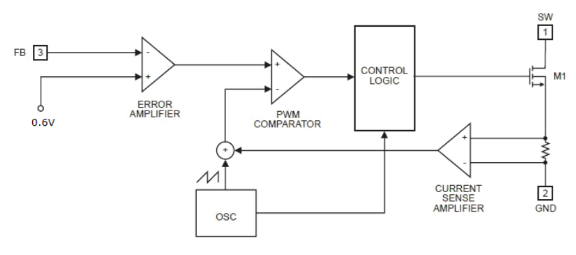
\includegraphics[width=0.7\textwidth]{figuras/circuitomt3608.png}
    \caption{Circuito interno del chip \emph{MT3608}}
    \label{fig:circuitomt3608}
\end{figure}

El transistor M1 es el switch que se observa en el diagrama del circuito boost, que se manipula mediante un bloque lógico de control conectado a su entrada de compuerta.

El control comienza con el amplificador de error, que compara la entrada de feedback del chip (una muestra de la tensión de salida final), con una señal de 0,6 voltios muy estable. A la salida de este amplificador tenemos una señal proporcional al error de la tensión en la carga. El diseñador debe procurar que cuando la tensión en la carga se encuentre en su valor óptimo, la entrada de feedback debe ser igual a esos 0,6 voltios, para que en esa situación la salida sea constante y no afecte a la modulación.

Cuando la salida es mayor a su valor esperado ($V_{FB} > V_{REF}$), el comparador de error reacciona disminuyendo la señal de error, mientras que cuando la salida es menor ($V_{FB} < V_{REF}$), la señal de error aumenta. Finalmente, si ambas entradas son iguales ($V_{FB} = V_{REF}$), el error será una señal constante, como se mencionó anteriormente. Todo lo anterior se refleja en la siguiente imagen:

\begin{figure}[htbp]
    \centering
    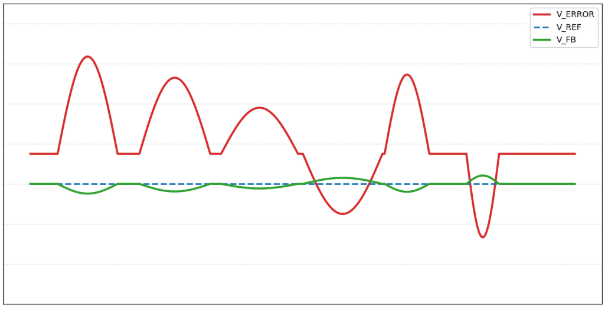
\includegraphics[width=0.5\textwidth]{figuras/tensionesamperror.png}
    \caption{Gráfico explicativo del comportamiento del amplificador de error}
    \label{fig:tensionesamperror}
\end{figure}

Este valor de error ingresa en el amplificador comparador PWM junto a una señal diente de sierra generada por un oscilador, para que a su salida se obtenga la señal de control que finalmente manipule los estados del transistor M1. El mismo oscilador diente de sierra es quien activa el pulso de la compuerta, cerrando así la llave y permitiendo que la bobina se cargue. Mientras la tensión de error supere a la señal del oscilador, el pulso se mantiene activo. Cuando la señal diente de sierra supera a la señal de error, el pulso se desactiva abriendo la llave y dejando que la bobina se descargue hasta el próximo ciclo. 

\begin{figure}[htbp]
    \centering
    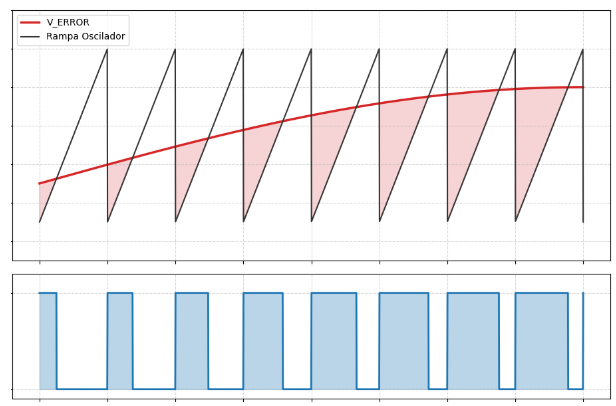
\includegraphics[width=0.5\textwidth]{figuras/pwm.png}
    \caption{Modulación por ancho de pulso (PWM)}
    \label{fig:pwm}
\end{figure}

Si la bobina pasa más tiempo cargándose (ciclo de trabajo grande), la tensión que genera al momento de descargarse aumentará junto con la tensión de salida, y si pasa más tiempo descargándose (ciclo de trabajo pequeño), la tensión de descarga será menor disminuyendo la salida final.

De todo este análisis se puede inferir la siguiente conclusión: Si la tensión de salida decae, el ancho del pulso, y por consiguiente la tensión de salida, aumentan. Por el contrario, si ocurre un exceso de voltaje en la carga, tanto el ancho de pulso como la tensión de salida disminuyen.

Por último, en el diagrama de bloques se observa un último amplificador que cumple dos funciones importantes: el sensor de corriente. Por un lado, actúa como sistema de protección, detectando situaciones en las que la corriente a través del switch aumenta a valores peligrosos. Para ello, lee la tensión sobre una resistencia del orden de los miliohmios (para interferir lo menos posible con el circuito original) y, ante un pico indeseado, envía una señal a la lógica de control que abre la llave para evitar la destrucción del circuito. Por otro lado, durante el funcionamiento normal, esta misma lectura de corriente se suma a la señal del oscilador para alimentar al comparador PWM, esto permite que el chip ajuste el ancho de pulso instantáneamente en cada ciclo, garantizando estabilidad ante variaciones rápidas de carga. 

Con todo el funcionamiento explicado, podemos pasar a mostrar el diagrama de pines:

\begin{figure}[htbp]
    \centering
    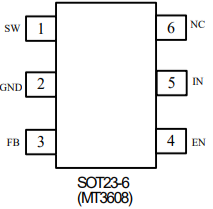
\includegraphics[width=0.3\textwidth]{figuras/mt3608pinout.png}
    \caption{Diagrama de pines del módulo \emph{MT3608}}
    \label{fig:mt3608pinout}
\end{figure}

\begin{itemize}

\item SW: Es el pin que conecta al MOSFET M1 con el circuito boost externo (El drenador del transistor).

\item GND: Tensión de referencia.

\item FB: Tensión de feedback. Es una muestra de la tensión de salida que luego se compara con los 0,6 V internos.

\item EN: Habilitación del chip.

\item IN: Tensión de entrada. 

\item No se utiliza.

\end{itemize}

A continuación se muestran algunos gráficos de funcionamiento típico.

Regulación de carga: Indica la corriente máxima que puede entregar a una carga de determinado valor de tensión (en este caso, con 500 mA es más que suficiente para suplir las exigencias del \emph{ESP32}).

\begin{figure}[htbp]
    \centering
    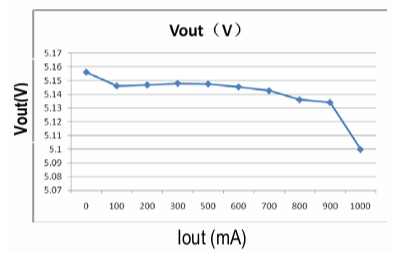
\includegraphics[width=0.5\textwidth]{figuras/regulacioncarga.png}
    \caption{Regulación de carga del \emph{MT3608}}
    \label{fig:regulacioncarga}
\end{figure}

Frecuencia de conmutación según tensión de entrada: Vemos que en nuestro caso llegamos a valores de entre 0,9 y 1 Mhz. No es el ideal de 1,2 que se describió anteriormente, pero a fines prácticos sirve para mitigar lo suficiente el ripple de salida.

\begin{figure}[H]
    \centering
    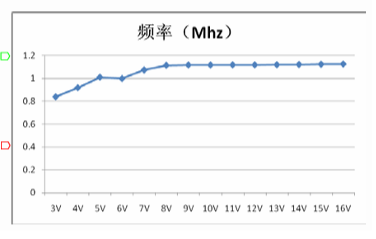
\includegraphics[width=0.5\textwidth]{figuras/freqvsvin.png}
    \caption{Frecuencia vs Tensión de entrada en el chip \emph{MT3608}}
    \label{fig:freqvsvin}
\end{figure}

Eficiencia vs tensión de entrada: Mientras mayor la tensión de entrada, más eficiente el circuito. En este caso se a roza el 90\%

\begin{figure}[H]
    \centering
    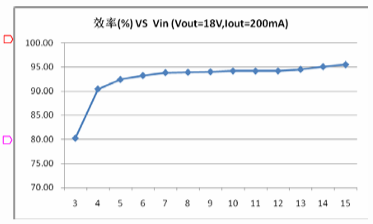
\includegraphics[width=0.5\textwidth]{figuras/eficiencia.png}
    \caption{Eficiencia vs Tensión de entrada en el chip \emph{MT3608}}
    \label{fig:eficiencia}
\end{figure}

A continuación se muestra el circuito que viene en los módulos \emph{MT3608} comerciales, que incluyen el circuito boost externo:

\begin{figure}[htbp]
    \centering
    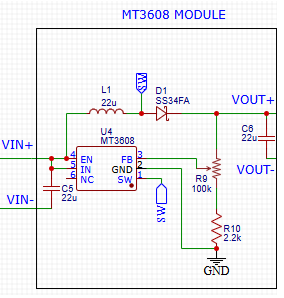
\includegraphics[width=0.5\textwidth]{figuras/mt3608placa.png}
    \caption{Circuito comercial de los módulos \emph{MT3608}}
    \label{fig:mt3608placa}
\end{figure}

El circuito comienza con los pines de entrada y habilitación cortocircuitados y conectados a la tensión de 3,7 voltios provenientes de la pila, ya que al igual que con el \emph{TP4056}, no se requiere deshabilitar manualmente el integrado. A su vez, el pin de entrada se conecta a uno de los terminales de la bobina de 22 uH, para cargarla en los momentos en que la llave se encuentra cerrada.

El pin de switch (el drenador del MOSFET), se conecta al otro terminal de la bobina y al ánodo de un diodo de alta velocidad, como indica el modelo del circuito boost expuesto anteriormente.

Finalmente, el pin de feedback se conecta a un potenciómetro de 100 kΩ en serie con una resistencia de 2,2 kΩ. El valor de este potenciómetro se ajusta con un tornillo externo para seleccionar el valor de tensión a la salida (dado por la señal obtenida en el amplificador de error). Se colocan esos valores de resistencia para limitar la tensión de salida a un mínimo de 0,6 V y un máximo absoluto de 28 V.

Se observa también el capacitor C6 del circuito boost, un capacitor C5 de desacople, y el pin de GND conectado a la masa del circuito.

\keyword {Componentes a utilizar en el dispositivo final}

Con todo el sistema explicado, se listan a continuación todos los materiales necesarios para construir los circuitos de alimentación:

\begin{itemize}

\item 4 Borneras de 2 terminales
\item 4 Capacitores  cerámicos de 100 nF (para reducir el ruido).
\item 2 Baterías de Litio de 3,7 voltios con 3000 mAh de energía.
\item 2 Capacitores electrolíticos de 10 uF (para reducir picos de corriente).
\item 2 Módulos de carga \emph{TP4056} comerciales (con chips \emph{DW01A} y \emph{FS8205A} incluidos).
\item 2 Módulos elevadores \emph{MT3608} comerciales.
\item 2 PCBs de las dimensiones adecuadas.
\item 2 Resistencias de 1/4 de vatio de 160 ohmios para los diodos LED.
\item 2 Switches para encendido del dispositivo.
\item 2 Zócalos o portapilas individuales.
\item 1 Bornera de 3 terminales.
\item 1 Diodo LED azul.
\item 1 Diodo LED infrarrojo emisor.
\item Zócalos hembra-macho para portar la \emph{ESP32-CAM} en la PCB

\end{itemize}


\section{Costo total de desarrollo}

(Tabla hecha por naty)
